\documentclass[11pt,oneside,letterpaper]{article}

% graphicx package, useful for including eps and pdf graphics
\usepackage{graphicx}
\DeclareGraphicsExtensions{.pdf,.png,.jpg}

% basic packages
\usepackage{color} 
\usepackage{parskip}
\usepackage{float}
\usepackage[hyphens]{url}   % allow breaks after “/”, “-”, …
\usepackage{xurl}           % (optional) adds even more break points
\usepackage[hidelinks,breaklinks]{hyperref}


% text layout
\usepackage{geometry}
\geometry{textwidth=15cm} % 15.25cm for single-space, 16.25cm for double-space
\geometry{textheight=22cm} % 22cm for single-space, 22.5cm for double-space

% helps to keep figures from being orphaned on a page by themselves
\renewcommand{\topfraction}{0.85}
\renewcommand{\textfraction}{0.1}

% bold the 'Figure #' in the caption and separate it with a period
% Captions will be left justified
\usepackage[labelfont=bf,labelsep=period,font=small]{caption}

% review layout with double-spacing
%\usepackage{setspace} 
%\doublespacing
%\captionsetup{labelfont=bf,labelsep=period,font=doublespacing}

% cite package, to clean up citations in the main text. Do not remove.
\usepackage{cite}
%\renewcommand\citeleft{(}
%\renewcommand\citeright{)}
%\renewcommand\citeform[1]{\textsl{#1}}

% Remove brackets from numbering in list of References
\renewcommand\refname{\large References}
\makeatletter
\renewcommand{\@biblabel}[1]{\quad#1.}
\makeatother

\usepackage{authblk}
\renewcommand\Authands{ \& }
\renewcommand\Authfont{\normalsize \bf}
\renewcommand\Affilfont{\small \normalfont}
\makeatletter
\renewcommand\AB@affilsepx{, \protect\Affilfont}
\makeatother

% notation
\usepackage{amsmath}
\DeclareMathOperator*{\argmax}{arg\,max}
\usepackage{amssymb}
\usepackage{graphicx}
\newcommand{\virus}{\mathbf{x}}						% virus coordinate
\newcommand{\serum}{\mathbf{y}}						% serum coordinate
\newcommand{\viruses}{\mathbf{X}}					% set of virus coordinates
\newcommand{\sera}{\mathbf{Y}}						% set of serum coordinates
\newcommand{\ve}{v}									% virus avidity
\newcommand{\se}{s}									% serum potency
\newcommand{\ves}{\mathbf{v}}						% set of virus avidities
\newcommand{\ses}{\mathbf{s}}						% set of serum potencies
\newcommand{\point}{f_{\scriptscriptstyle \vert}}	% point likelihood
\newcommand{\threshold}{f_{\textstyle \lrcorner}}	% threshold likelihood
\newcommand{\interval}{f_{\sqcup}}					% interval likelihood
\newcommand{\mdssd}{\varphi}						% MDS standard deviation
\newcommand{\virussd}{\sigma_x}						% virus / diffusion standard deviation
\newcommand{\serumsd}{\sigma_y}						% serum standard deviation
\newcommand{\drift}{\mu}							% drift / advection
\newcommand{\tree}{\tau}							% phylogeny
\newcommand{\vn}{n}									% number of viruses
\newcommand{\sn}{k}									% number of sera
\newcommand{\normal}{\mathcal{N}}					% normal distribution
\newcommand{\bwithin}{\beta_w}		% within clade drift coefficient
\newcommand{\bsister}{\beta_s}		% sister clade drift coefficient
\newcommand{\bother}{\betZ_t}			% across clade drift coefficient
\newcommand{\incclade}[1]{y_\mathrm{#1}}
\newcommand{\driftclade}[1]{x_\mathrm{#1}}
\newcommand{\States}{[M]} % = {1,\dots,M}
\setlength{\arraycolsep}{2pt}
\newcommand{\smalltwomatrix}[2]{\scriptsize \Big( \begin{matrix} #1 \\ #2 \end{matrix} \Big)}				% pretty inline matrix 
\newcommand{\smallfourmatrix}[4]{\scriptsize \Big( \begin{matrix} #1 & #2 \\ #3 & #4 \end{matrix} \Big)}	% pretty inline matrix 
\newcommand{\twomatrix}[2]{\left( \begin{matrix} #1 \\ #2 \end{matrix} \right)}								% pretty inline matrix 
\newcommand{\fourmatrix}[4]{\left( \begin{matrix} #1 & #2 \\ #3 & #4 \end{matrix} \right)}		% pretty inline matrix 
\usepackage{booktabs}

%%% TITLE %%%
\title{\vspace{1.0cm} \Large \bf 
Hidden Markov Models Detect Pango Lineage Ancestry of Recombinant SARS-CoV-2 Sequences 
}

\author[1]{Nobuaki Masaki}
\author[2]{Trevor Bedford}

\affil[1]{Department of Biostatistics, University of Washington, Seattle, WA}
\affil[2]{Vaccine and Infectious Disease Division, Fred Hutch Cancer Center, Seattle, WA}

\date{}

\begin{document}

\maketitle

%%% ABSTRACT %%%
\begin{abstract}
When individuals are co-infected with two SARS-CoV-2 lineages, homologous recombination can generate mosaic genomes carrying mutations from both parental lineages. There are a variety of methods developed to detect recombinant sequences and their parental lineages in a surveillance-scale dataset comprised of millions of SARS-CoV-2 genomes. However, these methods often rely on user-defined settings, such as the probability that a recombination breakpoint occurs between adjacent positions on the query sequence. In this study, we devise a hidden Markov model that detects recombinant SARS-CoV-2 sequences and identifies their parental lineages within a test set of sequences collected over a week-long window.  Our method does not depend on user-defined parameters and can accommodate de novo mutations on the query sequence that are not present in the inferred parental lineages. To achieve this, we use maximum likelihood to estimate parameters that characterize the transition and emission probabilities in our hidden Markov model. Applying our method to 440,307 SARS-CoV-2 sequences sampled in England between September 2020 and March 2024, we detect 7,619 recombinant sequences corresponding to 1.73\% (95\% CI: [1.69\%, 1.77\%]) of all sampled sequences. We show a positive association between the proportion of query sequences detected as recombinant in each week and community SARS-CoV-2 prevalence. This is consistent with higher prevalence increasing co-infection risk and promoting the emergence of recombinant sequences. We further observe localized clusters of recombination breakpoints within Spike and in intergenic regions.
\end{abstract}

% Recombinant SARS-CoV-2 viruses can emerge when an individual is coinfected with multiple variants of the virus. However, it can be challenging to identify recombinant SARS-CoV-2 sequences and their parental lineages among thousands of samples. We developed a novel inferential framework capable of determining the parental Pango lineage at each position of a putative recombinant SARS-CoV-2 sequence, using a reference set of sequences and associated Pango lineages.

%%% IMPACT %%%
% Combined evolutionary and antigenic analysis shows that human influenza viruses differ dramatically in rates of antigenic drift and these rates significantly impact seasonal incidence patterns.

\pagebreak

%%% INTRODUCTION %%%
\section{Introduction}

Recombination is thought to occur in coronaviruses via a copy-choice mechanism in which the viral RNA-dependent RNA polymerase switches template strands during negative strand synthesis \cite{chrisman_indels_2021}. When hosts are co-infected by multiple SARS-CoV-2 lineages, this template switching results in recombinant genomes sharing mutations from both lineages \cite{tremeaux_sars-cov-2_2023}.

One of the most significant recombinant lineages that emerged during the pandemic is XBB. Phylogenetic analysis indicates that this lineage was derived from a recombination event between two Omicron lineages (BJ.1 and BM.1.1.1) \cite{tamura_virological_2023}. Furthermore the XBB.1 Spike, harboring substitutions derived from both BJ.1 and BM.1.1.1, was associated with a 30-fold reduction in neutralization by BA.2 breakthrough sera. The effects of individual substitutions (e.g., V83A, Y144del, Q183E, R346T, L368I, V445P, F486S, F490S) were modest, yielding 3-fold reductions in neutralization \cite{tamura_virological_2023}.

Additionally, the effective reproduction number of XBB was estimated to be 1.23 and 1.20 times higher than its parental lineages BJ.1 and BM.1.1.1, respectively, using epidemic data from late 2022 \cite{tamura_virological_2023}. XBB.1.5 reached a peak lineage frequency of 55\% globally in epidemiological week~12 of 2023 \cite{erkihun_current_2024}. In the United States, XBB.1.5 reached a peak lineage frequency of 84.1\% by April~1,~2023 \cite{ma_genomic_2023}. Because recombination can combine mutations from different SARS-CoV-2 lineages that jointly confer a growth advantage, systematic surveillance and robust statistical detection of recombinant lineages are crucial.

A wide range of computational approaches have been developed to detect recombination in viruses. Broadly, similarity methods such as SimPlot visualize how a query sequence’s similarity shifts across the genome relative to putative parental lineages \cite{samson_simplot_2022, salminen_identification_1995}. RDP4 examines all triplets within a set of sequences and applies a suite of tests (e.g., GENECONV, MaxChi, Bootscan, 3SEQ) to detect recombination breakpoints and assign parental sequences \cite{martin_rdp4_2015, sawyer_statistical_1989, posada_evaluation_2001, lam_improved_2018}. However, the number of comparisons is cubic with respect to the sample size, which is infeasible for large-scale datasets.

% GENECONV detects unusually long tracts of identity between sequence pairs via permutation tests. MaxChi calculates a \(\chi^2\) statistic based on discordant sites between the query sequence and two parental lineages to the left and right of each breakpoint. Bootscan builds bootstrapped phylogenetic trees in sliding windows to detect parental switches; 3SEQ tests whether a candidate sequence forms a mosaic of two others by identifying clusters of sites where it matches one parent over the other, using an exact nonparametric permutation test. 

Phylogeny-based methods such as GARD detect breakpoints by fitting phylogenies to alignment segments and comparing model fit across candidate partitions \cite{kosakovsky_pond_gard_2006}. The repeated tree-fitting and model-comparison steps are computationally intensive, so GARD is generally applied to downsampled alignments instead of surveillance-scale datasets comprising millions of genomes.

More recently, SARS-CoV-2-specific tools have been designed to operate on surveillance-scale datasets. Bolotie uses a hidden Markov model (HMM) where the latent states represent SARS-CoV-2 lineages \cite{varabyou_rapid_2021}. The Viterbi algorithm is used to assign a parental lineage to each position. RIPPLES identifies candidate recombinant sequences by scanning a global mutation-annotated phylogeny for unusually long branches that may represent recombination events \cite{turakhia_pandemic-scale_2022}. For each candidate recombinant sequence, RIPPLES partitions the genome into multiple segments and re-places each onto the global phylogeny using maximum parsimony. RecombinHunt compares segment‑wise mutation patterns on a query sequence to lineage‑specific profiles \cite{alfonsi_data-driven_2024}. It constructs a cumulative likelihood profile across the genome and uses the Akaike information criterion to choose between three models with zero, one, or two breakpoints.

Although these SARS‑CoV‑2–specific tools can be applied to surveillance‑scale datasets, each has method‑specific limitations. Bolotie’s HMM does not model de novo mutations or genotyping errors, which can result in spurious state switches when the query sequence harbors mutations absent from the mutation profile of its true lineage. The HMM’s transition probability is also user‑specified, making breakpoint detection sensitive to this choice. RIPPLES relies on a mutation‑annotated phylogeny. Uneven sampling and sequencing artifacts can inflate or deflate the long‑branch signal used to identify candidate recombinants. Moreover, the threshold for the long-branch signal is defined by the user, and the initial candidate set of recombinant sequences is sensitive to this chosen cutoff. RecombinHunt relies on several hard evidence gates (e.g., declaring a genome non‑recombinant when it differs from the most likely lineage by two or fewer mutations). These thresholds are likewise sensitive to de novo mutations and genotyping errors. Finally, both RIPPLES and RecombinHunt permit at most two breakpoints, even though recombinant lineages with more breakpoints have been detected.

In this paper, we develop a method to detect recombinant SARS‑CoV‑2 sequences within a test set of sequences collected over a short interval (a few days to a week). Our method employs an HMM inspired by the Li and Stephens model \cite{li_modeling_2003} that accounts for de novo mutations and genotyping errors in both recombinant and non‑recombinant sequences. For each test sequence, we estimate a pseudo-frequency for observing alleles absent from the parental lineage at a position, and the lineage-transition probability between consecutive sites. We implement an efficient version of the forward algorithm to speed up estimation of these frequencies (see Supplementary Materials). We then infer the local Pango lineage ancestry, defined as the sequence of Pango lineages ancestral at each genomic position of the test sequence, using lineage-specific nucleotide frequencies computed from prior sequences. We classify a test sequence as a recombinant if the inferred local Pango lineage ancestry contains one or more lineage transitions. Our method does not rely on a phylogeny nor any user‑defined parameters, and can accommodate any number of breakpoints.

We evaluate performance in a simulation where we generated synthetic recombinant and control genomes from SARS-CoV-2 sequences sampled between January and March 2022. We report sensitivity and specificity for classifying sequences as recombinant or non-recombinant, the fraction of synthetic sequences for which we recovered the true parental lineages, and mean distances between true and inferred breakpoints.

We apply our method to 440,307 SARS‑CoV‑2 genomes from GenBank, sampled in England between September 2020 and March 2024 \cite{benson_genbank_2013}. We assign these sequences to contiguous, non-overlapping test windows. We detect 7,619 recombinant sequences, corresponding to 1.73\% (95\% CI: [1.69\%, 1.77\%]) of all sequences. We show that the proportion of sequences detected as recombinant in each test window is positively associated with community SARS-CoV-2 prevalence estimated in the UK Office of National Statistics (ONS) Coronavirus Infection Survey \cite{pouwels_community_2021}. This is consistent with higher prevalence increasing co-infection risk and thereby promoting the emergence of recombinant sequences. We further find a positive association between the number of detected recombinants stratified by unique parental lineage pairs (e.g., BA.1.1--BA.2) and an estimate of expected counts based on co-infection dynamics between these lineage pairs. Finally, we observe enrichment of detected recombination breakpoints using our method within Spike and in intergenic regions.

%%% METHODS %%%
\section{Materials and methods}

Figure \ref{fig:method} summarizes our workflow for detecting the local Pango lineage ancestry of SARS-CoV-2 sequences from GenBank. In this section, we describe each component of our method in detail. 

\begin{figure}[H]
  \centering
  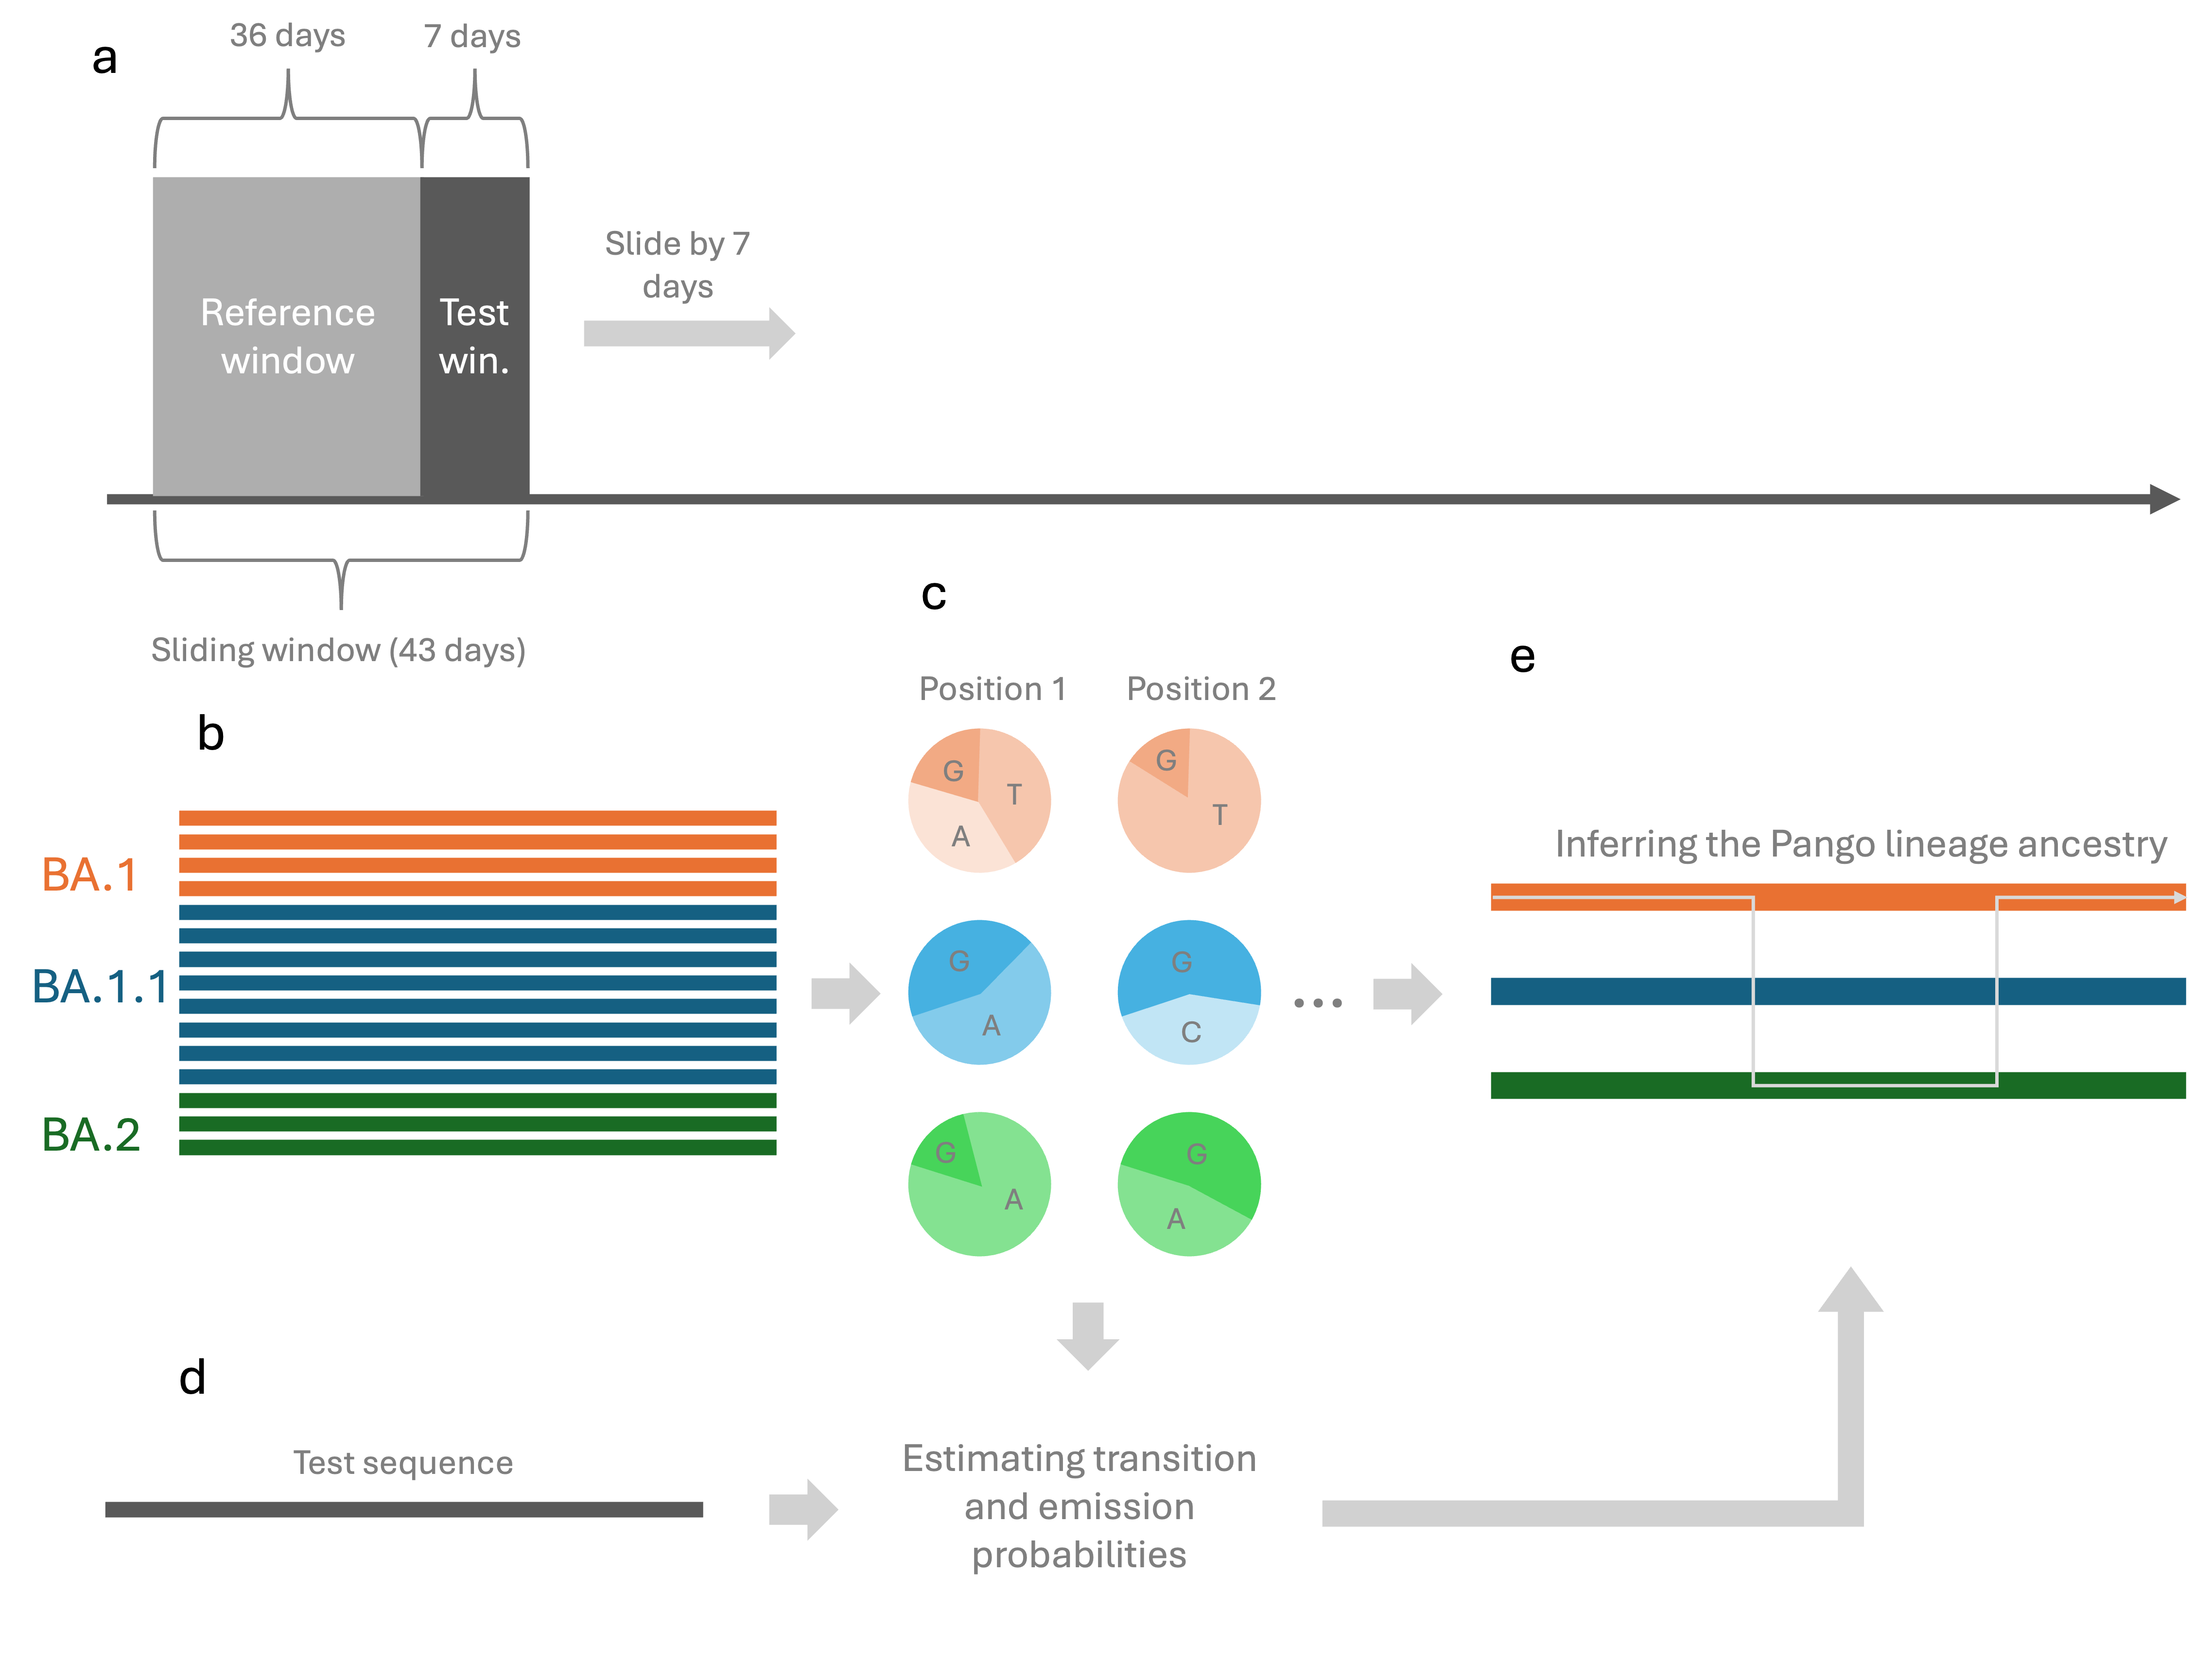
\includegraphics[width=0.9\textwidth]{figures/hmm/methods6.png}
  \caption[Overview]{Overview of methods. We first organize SARS-CoV-2 sequences collected in England between September 2020 and March 2024 into sliding windows of 43 days, which are advanced by 7 day increments (panel a). In each sliding window, the first 36 days and last 7 days respectively comprise the reference window and test window. Sequences collected during the reference window comprise the reference set of sequences containing the mutational profile of each Pango lineage (panel b). We next calculate the nucleotide frequency matrix containing per-position allele frequencies for each Pango lineage in the reference set (panel c). For each test sequence collected during the test window (panel d), we use maximum likelihood to estimate frequencies that parameterize the transition and emission probabilities of our HMM. We then use the Viterbi algorithm to infer the local Pango lineage ancestry for this sequence (panel e).}
  \label{fig:method}
\end{figure}

% We then use the Viterbi algorithm to infer the local Pango lineage ancestry for this sequence (panel e), which depends on the estimated pseudo-frequency and transition probability from the previous step.

\subsection{Obtaining SARS-CoV-2 sequences and clustering Pango lineages}\label{subsec:data}

We obtained SARS-CoV-2 sequences and associated metadata from GenBank, processed using the Nextstrain pipeline \cite{hadfield_nextstrain_2018}. After filtering for sequences collected in England between September 2020 and March 2024, we clustered Pango lineages based on their sequence count. Any Pango lineages with fewer than 10,000 sequences were collapsed into their parental lineage using unaliased Pango lineage names \cite{otoole_assignment_2021}. This was done iteratively to ensure that all collapsed Pango lineages contained at least 10,000 sequences. 
Lineages without a defined parent were grouped into a shared ``other" category. We collapsed 2,304 Pango lineages that existed during this period to 41 collapsed lineages (including the ``other" category). Unless otherwise specified, all mentions of Pango lineages refer to the collapsed lineages resulting from this procedure. 

\subsection{Reference and test sets}\label{subsec:reference_set}

From the sequences collected in England between September 2020 and March 2024, we generated sliding windows of reference and test set pairs. Each sliding window consisted of 43 days, and these windows were incremented by 7 days at a time to generate 185 sliding windows.

In each 43-day sliding window, the first 36 days define the reference window, and the last 7 days define the test window. Sequences collected during the reference and test windows respectively comprise the reference and test sets for this sliding window. 

If more than 100,000 sequences were collected during the reference window, we drew a random sample of 100,000 sequences and used this as the reference set. Similarly, if more than 3,000 sequences were collected during the test window, we drew a random sample of 3,000 sequences and used this as the test set. 

This process results in 185 pairs of reference and test sets. In the following sections, we describe our process for calculating the nucleotide frequency matrix for each reference set, and our HMM, which uses the nucleotide frequency matrix to infer the local Pango lineage ancestry for each sequence in the paired test set. 
 % These thresholds were chosen empirically to (i) keep the reference sets large enough to yield stable nucleotide-frequency estimates, (ii) provide a test set that captures a representative ``snapshot" of recombinants emerging within each 7-day period, and (iii) keep downstream HMM ancestry inference computationally tractable.
\subsection{Calculating the nucleotide frequency matrix}\label{subsec:freq_matrix}

For each of the 185 reference sets, we calculated a nucleotide frequency matrix that contains the frequency of each nucleotide (A, C, G, T) at every genomic position for each Pango lineage. Nucleotide frequencies were calculated by dividing nucleotide counts at each position by the total sequence count within each Pango lineage.  When calculating frequencies, we excluded all non-standard nucleotides (i.e., those other than A, C, G, T). If no sequences in a Pango lineage carried any of the standard nucleotides at a position, we assigned equal probabilities (0.25 each) to A, C, G, and T.

\subsection{Predicting the local Pango lineage ancestry}

The local Pango lineage ancestry of a SARS-CoV-2 sequence refers to the sequence of Pango lineages contributing ancestry to each genomic position of the SARS-CoV-2 sequence. 

If a sequence results from a recombination event between two sequences in two distinct Pango lineages, its local Pango lineage ancestry will consist of segments derived from these distinct lineages, with transitions between segments marking recombination breakpoints. Conversely, for non-recombinant sequences, the local Pango lineage ancestry will only contain a single parental lineage. It is important to note that the true local Pango lineage ancestry of a sequence in a test set is defined in relation to the Pango lineages present in the paired reference set. For example, lineages $L_1$, $L_2$, and $L_3$ may all be present in the paired reference set, with lineage $L_3$ arising from a recombination event between two sequences in lineages $L_1$ and $L_2$ respectively. Suppose that there is a sequence from lineage $L_3$ in the test set. In this case, the true local Pango lineage ancestry of this sequence will have $L_3$ as the lineage contributing ancestry at all genomic positions. 

We predict the local Pango lineage ancestry of all sequences in each test set using the nucleotide frequency matrix calculated from the corresponding reference set and an HMM inspired by the Li and Stephens model \cite{li_modeling_2003}.

This HMM jointly models the latent local Pango lineage ancestry and the observed nucleotide sequence for each test sequence. It does so by considering three key components: (i) the probability of each Pango lineage contributing ancestry at the first position (initial state probabilities), (ii) the probability of transitioning between different Pango lineages along the genome (transition probabilities), and (iii) the probability of observing each nucleotide at a given position, conditional on the Pango lineage (emission probabilities). Transitions between lineages correspond to recombination events. 
 
\subsection{Hidden Markov model to predict local Pango lineage ancestry}

In this section, we define the HMM used to predict the local Pango lineage ancestry of a sequence in any given test set. We henceforth refer to this sequence as our test sequence.

Let the genome length be denoted by $N$ and let $t \in \{1, 2, \dots, N\}$ index genomic positions. Our sequences are aligned, so all of our sequences have length $N$.

For our test sequence, we define the random variable for the parental Pango lineage at position $t$ as $Z_t$. $Z_t$ is supported on $\{1, 2, \dots, M\}$, where $M$ is the number of distinct Pango lineages contained in the paired reference set (the reference set paired with the test set from which the test sequence is drawn). Each value of $\{1, 2, \dots, M\}$ corresponds to one of these Pango lineages. 

We further define, for the test sequence, the random variable for the observed nucleotide at position $t$ as $O_t$. $O_t$ is supported on \{$\text{A}, \text{C}, \text{G}, \text{T}\}$.

In the following sections, we define the three key components of this HMM, which are the initial state probabilities, the transition probabilities, and the emission probabilities.

\subsubsection{Initial state probabilities}

The initial state probabilities represent the probability of each Pango lineage being the parental lineage of the test sequence at the first genomic position. We define the initial state probability of Pango lineage $i$ ($i \in \{1, 2, \dots, M\}$) as $\pi_i = P(c_1 = i)$, where $c_1$ denotes the parental lineage of the test sequence at the first position. In our model, we set $\pi_i$ proportional to the frequency of lineage $i$ in the paired reference set. Let $n_i$ be the number of sequences assigned to lineage $i$ in the reference set, and let $n_{\text{total}} = \sum_{j=1}^M n_j$ be the total number of sequences across all $M$ lineages. Then,

\begin{align*}
    \pi_i = \frac{n_i}{n_{\text{total}}}, \quad i \in \{1, 2, \dots, M\}.
\end{align*}

\subsubsection{Transition probabilities}

Transition probabilities represent the probability that we will transition from one parental Pango lineage to another between consecutive positions on the test sequence. Here, transitions between Pango lineages correspond to recombination breakpoints. We define the transition probability from Pango lineage $i$ to Pango lineage $j$ as

\begin{align*}
a_{ij} = P(Z_{t+1} = j \mid Z_t = i), \quad i,j \in \{1, 2, \dots, M\}, \quad t \in \{1, 2, \dots, N-1\}.
\end{align*}

Here, $a_{ij}$ represents the probability that the parental Pango lineage of the test sequence changes from $i$ to $j$ between any consecutive positions on the genome. In our model, we set transition probabilities as

\begin{align*}
a_{ij} =
\begin{cases}
1-\lambda, & \text{if } i = j, \\
\frac{\lambda}{M - 1}, & \text{if } i \neq j.
\end{cases}
\end{align*}

$\lambda$ is the probability that there is a recombination breakpoint between consecutive positions on the genome. For the above formulation, we also assume that transitions between any two Pango lineages $i \neq j$ occur with the same probability. Because $\lambda$ is an unknown parameter, we later describe our method for estimating $\lambda$. 

% These transition probabilities are stored in a transition matrix $\mathbf{A}$, with entry $a_{ij}$ located at row $i$, column $j$. This yields the following structure for the transition matrix $\mathbf{A}$:

% \begin{align*}
% \mathbf{A} =
% \begin{bmatrix}
% \sigma & \frac{1-\sigma}{M-1} & \cdots & \frac{1-\sigma}{M-1} \\
% \frac{1-\sigma}{M-1} & \sigma & \cdots & \frac{1-\sigma}{M-1} \\
% \vdots & \vdots & \ddots & \vdots \\
% \frac{1-\sigma}{M-1} & \frac{1-\sigma}{M-1} & \cdots & \sigma
% \end{bmatrix}.
% \end{align*}

\subsubsection{Emission probabilities}

Emission probabilities of the HMM define the probability of observing each nucleotide (i.e., A, C, G, T) at a particular position on the test sequence, conditional on the parental Pango lineage at that position. We define the emission probability of observing nucleotide $k$ at position $t$, conditional on the parental Pango lineage being $i$ at position $t$, as

\begin{align*}
    b_{i,t}(k) = P(O_t = k|Z_t = i), \quad k \in \{\text{A}, \text{C}, \text{G}, \text{T}\}, \quad i \in \{1, 2, \dots, M\}, \quad t \in \{1, 2, \dots, N\}.
\end{align*}

$b_{i,t}(k)$ depends on the nucleotide frequency matrix calculated from the paired reference set. We use $f_{i,t}(k)$ to denote the frequency of nucleotide $k$ at position $t$ in Pango lineage $i$ in the paired reference set. To adjust for possible mutations and genotyping errors that could occur on the test sequence, we apply a pseudo-frequency $\epsilon$. Specifically, we let

\begin{align*}
b_{i,t}(k) = \frac{f_{i,t}(k) + \epsilon}{1 + 4\epsilon}.
\end{align*}

The pseudo-frequency $\epsilon$ assigns a non-zero probability of observing a nucleotide at position $t$, when the parental Pango lineage at $t$ contains no sequences that have this nucleotide in the reference set. We want to allow for this non-zero probability in case the test sequence has acquired a mutation (or genotyping error) at position $t$ that leads to an observed nucleotide that is not contained in the Pango lineage. A small value of $\epsilon$ allows occasional mutations or genotyping errors without forcing a lineage switch in the inferred local Pango lineage ancestry. Because $\epsilon$ is an unknown parameter, we describe our method for estimating $\epsilon$ in the following section.

We assume that positions with non-ACGT calls contain no information about the true nucleotide and assign an emission probability of 1 across all parental Pango lineages.

\begin{table}[ht]
\centering
\begin{tabular}{ll}
\toprule
Symbol & Description \\
\midrule
$N$ & Genome length \\
$M$ & Number of Pango lineages in the reference set \\
$Z_t$ & Parental Pango lineage at position $t$ \\
$O_t$ & Observed nucleotide at position $t$ \\
$\lambda$ & Transition probability \\
$\epsilon$ & Pseudo-frequency for emissions (accounts for mutations and genotyping errors) \\
$a_{ij}$ & Transition probability from lineage $i$ to lineage $j$ \\
$b_{i,t}(k)$ & Emission probability of nucleotide $k$ at $t$ given $Z_t=i$ \\
$f_{i,t}(k)$ & Frequency of nucleotide $k$ at $t$ in lineage $i$ in the reference set \\
$\pi_i$ & Initial state probability that $c_1=i$ \\
\bottomrule
\end{tabular}
\caption[Summary of symbols used in the hidden Markov model]{Summary of symbols used in the HMM.}
\end{table}

\subsection{Maximum likelihood estimation of parameters in the hidden Markov model}\label{sec:MLEHMM}

We have two unknown parameters in our HMM. $\lambda$ represents the probability that the parental Pango lineage changes between consecutive positions and $\epsilon$ is our psuedo-frequency, which adjusts emission probabilities to accommodate mutations or genotyping errors on the test sequence.

To perform maximum likelihood estimation on these two parameters, we first obtain the probability of the observed nucleotide sequence of the test sequence, conditional on these two parameters. In this section, we describe the procedure we use to obtain this probability.

Using the transition and emission probabilities described in the previous sections, it is relatively straightforward to obtain the joint probability of a candidate local Pango lineage ancestry and the observed nucleotide sequence for a test sequence. Let $i_{1:N} = (i_1,i_2,\hdots,i_N) \in\States^N$ be a candidate local Pango lineage ancestry and $k_{1:N} = (k_1,k_2,\hdots,k_N)$ be the observed nucleotide sequence of this test sequence. Finally, let $Z_{1:N} = (Z_1,Z_2,\hdots,Z_N)$ and $O_{1:N} = (O_1,O_2,\hdots,O_N)$. Then,

\begin{align*}
    P(Z_{1:N}=i_{1:N},\,O_{1:N}=k_{1:N}\mid \lambda,\epsilon)
    = \pi_{i_1}\,\Bigg(\prod_{t=1}^{N-1} a_{i_t i_{t+1}}\Bigg)
    \Bigg(\prod_{t=1}^{N} b_{i_t,t}(k_t)\Bigg).
\end{align*}

To obtain the marginal probability of the observed nucleotide sequence, we can simply sum up this joint probability across all possible local Pango lineage ancestries, as shown below.

\begin{align*}
    P(O_{1:N}=k_{1:N}\mid \lambda,\epsilon)
    = \sum_{i_{1:N}\in\States^N} 
    \pi_{i_1}\,\Bigg(\prod_{t=1}^{N-1} a_{i_t i_{t+1}}\Bigg)
    \Bigg(\prod_{t=1}^{N} b_{i_t,t}(k_t)\Bigg),
\end{align*}

This procedure can be done efficiently using the forward algorithm described by Rabiner \cite{rabiner_tutorial_1989}. We implemented an efficient version of the forward algorithm that computes the induction step in $\mathcal{O}(M)$ time compared to the normal $\mathcal{O}(M^2)$ time (see supplementary materials). We can maximize this marginal probability with respect to our two parameters to obtain our maximum likelihood estimates, as shown below.

\begin{align*}
    \hat\lambda, \hat\epsilon = \argmax_{\lambda,\epsilon}P(O_{1:N} = k_{1:N} \mid\lambda,\epsilon).
\end{align*}

Maximum likelihood estimation of $\lambda$ and $\epsilon$ is done for each test sequence. Optimization was carried out with the limited-memory BFGS algorithm subject to box constraints, using \texttt{scipy.optimize.minimize} (\texttt{method = "L-BFGS-B"})\,\cite{virtanen_scipy_2020}. Our efficient forward algorithm results in a large reduction in computation time, because the marginal likelihood is evaluated repeatedly during L-BFGS-B optimization.

During numerical optimization, we reparameterize $\lambda$ to $\tau = \lambda(N-1)$, which represents the expected number of transitions for the test sequence. Furthermore, we optimized $\epsilon$ on the log scale and later exponentiated to obtain our estimate in the original scale. The search was initialized at $(\log(\epsilon),\tau) = (\log(0.005),\,1)$ and restricted to the intervals $\log(\epsilon) \in [\log(10^{-8}),\,\log(0.02)]$ and $\tau \in [0,\,3]$. The reparameterization of $\lambda$ to $\tau$ was done to avoid possible numerical instabilities that might arise when trying to optimize $\lambda$ directly, because we expect $\lambda$ to be close to zero. We similarly optimized $\epsilon$ in the log scale because we expect $\epsilon$ to be close to zero. 

We chose the upper bound of three for $\tau$ because most discovered recombinant lineages were detected to have three or fewer breakpoints. However, this does not prevent the inferred local Pango lineage ancestry from having more than three breakpoints. 

\subsection{Obtaining the most likely sequence of Pango lineage ancestry}\label{sec:Viterbi}

We apply the Viterbi algorithm \cite{rabiner_tutorial_1989} to each test sequence to infer the most probable sequence of parental Pango lineage states along the genome,

\begin{align*}
\hat{i}_{1:N} = (\hat{i}_1, \ldots, \hat{i}_N).
\end{align*}

This represents the inferred local Pango lineage ancestry for this test sequence. Transitions between Pango lineage ancestries represent inferred recombination breakpoints.

When applying the Viterbi algorithm, we use our maximum likelihood estimates of the two frequencies, $\lambda$ and $\epsilon$, described in earlier sections. Specifically, we compute the sequence of Pango lineage ancestry that maximizes the joint probability of the ancestry path and the observed nucleotide sequence, given our maximum likelihood estimates. In other words,

\begin{align*}
\hat{i}_{1:N} 
&= \argmax_{i_{1:N}\in [M]^N}
P(Z_{1:N}=i_{1:N},\, O_{1:N}=k_{1:N} \mid
\hat\lambda, \hat\epsilon).
\end{align*}

Note that because $P(O_{1:N}=k_{1:N} \mid
\hat\lambda, \hat\epsilon)$ does not depend on the local Pango lineage ancestry, the above is equivalent to maximizing the posterior probability of the local Pango lineage ancestry given the observed nucleotide sequence and our maximum likelihood estimates. In other words,

\begin{align*}
\hat{i}_{1:N} 
&= \argmax_{i_{1:N}\in [M]^N}
P(Z_{1:N}=i_{1:N} \mid O_{1:N}=k_{1:N},
\hat\lambda, \hat\epsilon).
\end{align*}


% \section{Obtaining the mean maximum posterior probability for each test sequence}\label{sec:MMPP}

% To quantify the confidence of our local ancestry inference, we computed the mean maximum posterior probability (MMPP) for each test sequence. This measure summarizes the model's certainty in assigning a Pango lineage ancestry individually for each genomic position. 

% For each genomic position $t \in \{1, \dots, N\}$, the posterior probability of lineage $i \in \{1, 2, \dots, M\}$ being the ancestral Pango lineage is denoted by $P(Z_t = i \mid O_1 = k_1, O_2 = k_2, \hdots, O_N = k_N,
% \hat\sigma, \hat\epsilon)$, which is computed using the forward-backward algorithm described by Rabiner \cite{rabiner_tutorial_1989}.

% Then, the MMPP is defined as

% \begin{align*}
% \text{MMPP} = \frac{1}{N} \sum_{t=1}^N \max_{1 \leq i \leq M} P(Z_t = i \mid O_1 = k_1, O_2 = k_2, \hdots, O_N = k_N,
% \hat\sigma, \hat\epsilon),
% \end{align*}

% where $\max_{1 \leq i \leq M} P(Z_t = i \mid O_1 = k_1, O_2 = k_2, \hdots, O_N = k_N,
% \hat\sigma, \hat\epsilon)$ is the highest posterior probability among all lineages at position $t$.

% The MMPP should be interpreted with caution, because it does not capture the model's confidence in the predicted sequence of local Pango lineage ancestry for this test sequence. Instead, it offers a position-wise summary of posterior certainty, reflecting how strongly the model favors any one lineage at each site, irrespective of the overall path of predicted ancestry. A high MMPP indicates that the model consistently identifies a probable lineage at each position, but does not necessarily reflect the plausibility of the predicted sequence of local Pango lineage ancestry. 

\subsection{Simulation study}\label{sec:sim_recomb}

% Try to make the simulation study as close to the real data analysis as possible. So for example, we should be making the number of recombinant and non-recombinant sequences similar to a test set, to assess prevalence estimates

% We also want to assess whether confidence measures affect our estimates (prevalence and sensitivity, specificity)

% We should be assessing prevalence, sensitivity and specificity as a function of what? 

To assess our method’s ability to detect recombination and accurately assign local Pango lineage ancestries, we conducted a simulation study using synthetic SARS-CoV-2 sequences with known local Pango lineage ancestries. These synthetic sequences were generated from real SARS-CoV-2 genomes.

We generated these synthetic sequences using the reference set comprised of 14,599 SARS-CoV-2 sequences collected in England between November 6, 2022 and December 11, 2022. We simulated 1,000 recombinant sequences with two parental lineages and 1,000 control sequences with one parental lineage. 

Of the 1,000 recombinant sequences, 500 of them were generated using a single recombination breakpoint. To generate these sequences, we randomly sampled two parental sequences from different Pango lineages in the reference set and copied nucleotides from one parent up to a breakpoint randomly chosen on the genome, and from the other parent thereafter. The remaining 500 recombinant sequences were generated using two breakpoints. For these sequences, we again sampled two parental sequences from different Pango lineages. We chose two breakpoints randomly from all possible breakpoint combinations on the genome and inserted a middle segment from one sequence between these breakpoints, replacing the corresponding region in the genome of the other sequence. 

When a synthetic recombinant sequence differed by less than two mutations from one of its parental sequences, we discarded this sequence and repeated the sequence generation process. To mimic mutations, we drew the mutation count from an empirical distribution obtained by tallying nucleotide substitution counts on each branch of a tree containing one tip per Pango lineage \cite{hadfield_nextstrain_2018}. The empirical distribution of nucleotide substitution counts was right-skewed (n = 567; median = 2 [IQR 1–4]; mean = 3.45; 95th percentile = 8; range 1–70).

For each of the 2,000 synthetic sequences, we used the method described in Section \ref{sec:Viterbi} to predict the local Pango lineage ancestry. Emission probabilities for the HMM were based on the nucleotide frequency matrix calculated from the reference set of sequences collected between November 6, 2022 and December 11, 2022.

To evaluate performance, we conducted several quantitative assessments. First, we estimated the sensitivity and specificity of our method for detecting recombinant sequences. We classified a test sequence as a recombinant if the inferred local Pango lineage ancestry contained at least one lineage transition. Controls were treated as true negatives, and synthetic recombinants as true positives. 

Second, we estimated the mean position-by-position accuracy of the inferred local Pango lineage ancestry across synthetic sequences by comparing the inferred parental lineage at each genomic position to the true parental lineage. 

Third, we assessed whether the parental lineage(s) were correctly recovered for each synthetic sequence. Non-recombinant controls only have one parental lineage, while recombinants have two parental lineages. Both the mean position-by-position accuracy and the recovery rate of parental lineages were estimated separately for recombinant and non-recombinant sequences. 

For the sensitivity, specificity, and recovery rate of parental Pango lineages, we report 95\% exact binomial confidence intervals. For mean position-by-position accuracy, we calculated 95\% bootstrap confidence intervals by sampling 500 times with replacement from synthetic sequences (either from the set of recombinants or the set of non-recombinant sequences), calculating the mean position-by-position accuracy in each bootstrap sample, and taking the 2.5th and 97.5th percentiles of the bootstrapped estimates. 

% We further tested how accurately the method could estimate the proportion of recombinants, based on the predicted label. We can calculate the predicted-positive rate for a range of hypothetical true recombinant proportions in a similar set of test sequences. Denoting the estimated predicted-positive rate as $\widehat{\text{pred}}(\theta, \widehat{\text{Se}}, \widehat{\text{Sp}})$,

% \begin{align*}
%     \widehat{\text{pred}}(\theta, \widehat{\text{Se}}, \widehat{\text{Sp}}) = \theta \widehat{\text{Se}} + (1-\theta) (1-\widehat{\text{Sp}}),
% \end{align*}

% where $\theta$ represents the true prevalence, $\widehat{\text{Se}}$ represents the estimated sensitivity, and $\widehat{\text{Sp}}$ represents the estimated specificity. 

% We can also obtain a 95\% confidence interval for the predicted-positive rate: 

% \[
% \bigl[\ \theta\,\widehat{\text{Se}}_L + (1-\theta)\,(1-\widehat{\text{Sp}}_U),\ \ 
%         \theta\,\widehat{\text{Se}}_U + (1-\theta)\,(1-\widehat{\text{Sp}}_L)\ \bigr],
% \]

% where $[\widehat{\text{Se}}_L,\widehat{\text{Se}}_U]$ and $[\widehat{\text{Sp}}_L,\widehat{\text{Sp}}_U]$ are
% \v{S}id\'ak\text{-}adjusted marginal confidence intervals for sensitivity and specificity at level $1-\alpha'$ with $1-\alpha'=\sqrt{1-\alpha}$ (for $\alpha=0.05$, $1-\alpha'\approx 0.97468$), yielding nominal $1-\alpha=95\%$ joint coverage. This construction assumes the sampling errors of $\widehat{\text{Se}}$ and $\widehat{\text{Sp}}$ are independent, which is reasonable here because they are computed on disjoint positive and negative validation sets and no parameters are learned jointly from the combined data. 

Because the probability of correctly classifying a synthetic recombinant sequence is higher when the parental sequences of this sequence are less similar, we quantified the association between the sensitivity \(s(d)\) of the HMM and the genome-wide Hamming distance \(d\) between the parental sequences using a logistic regression:

\begin{align*}
  \text{logit}\!\bigl(s(d)\bigr)=\beta_{0}+\beta_{1}d.
  \label{eq:logistic_sensitivity}
\end{align*}

$\exp(\beta_{1})$ represents the multiplicative difference in the odds of detection for two synthetic recombinant sequences whose parental Hamming distances are one unit apart. To fit this logistic regression, we used the HMM's predicted label for all of the synthetic recombinants (1 if the model detected the sequence as a recombinant and 0 otherwise) as the outcome. 

To quantify breakpoint resolution, we calculated the distance between each inferred breakpoint and its corresponding true genomic position. We restricted analysis to synthetic recombinants whose detected breakpoint count matched the number of true breakpoints. For synthetic recombinants with one true breakpoint, we calculated the distance between the true and detected breakpoint. For synthetic recombinants with two true breakpoints, we ordered true and detected breakpoints 5' to 3', paired them positionally (1st with 1st, 2nd with 2nd), and calculated the distance between each pair. We then calculated the mean breakpoint distance separately for recombinants with one and two breakpoints.

We obtained 95\% confidence intervals for the mean breakpoint distance via nonparametric bootstrap. Specifically, we sampled recombinant sequences with replacement 500 times within each stratum (one and two breakpoints), calculated the mean breakpoint distance for each bootstrap sample within each stratum, and took the 2.5th and 97.5th percentiles of the bootstrapped estimates.

When the detected and true counts differed, we did not compute a distance. Instead we recorded the detected and true breakpoint counts per sequence and summarized mismatches in a contingency table.

\subsection{Real data analysis}\label{sec:methods_real_data}

We applied our method to the full set of SARS-CoV-2 sequences collected in England between September 2020 and March 2024. We describe how we obtain these sequences in Section \ref{subsec:data}. As described in Section \ref{subsec:reference_set}, sequences were divided into temporally matched reference and test sets using a 43-day sliding window, with a 36-day reference window followed by a 7-day test window. We inferred the local Pango lineage ancestry for sequences in each test window using the method described in Section \ref{sec:Viterbi}. If there were more than 3,000 sequences in a 7-day test window, we randomly sampled 3,000 sequences within the 7-day window and inferred the local Pango lineage ancestry for these sequences. Otherwise, we inferred the local Pango lineage ancestry for all sequences within the 7-day window. 

After obtaining the predicted local Pango lineage ancestry for test sequences, we classified any sequence with one or more lineage transitions as recombinant. For each 7-day test window, we counted the number of detected recombinant sequences and divided this by the total number of sequences in that test window. We refer to this quantity as the estimated recombinant proportion for the test window.

We hypothesized that the estimated recombinant proportion would be positively associated with community SARS-CoV-2 prevalence across test windows. This is because co-infection, which is required for the emergence of recombinant sequences, occurs more frequently when prevalence is higher. To evaluate our hypothesis, we compared the estimated recombinant proportion in each test window with community prevalence measured by the UK Office for National Statistics (ONS) Coronavirus Infection Survey \cite{pouwels_community_2021}. ONS provides prevalence estimates by date. For comparability, we computed the mean ONS prevalence within each test window and used this window-averaged prevalence in our analysis.

We further counted the number of detected recombinants across all windows, stratified by unique parental lineage pairs (e.g., BA.1.1\text{--}BA.2), and compared this to our estimated expected counts for each parental lineage pair based on co-infection dynamics, derived in Section \ref{sec:expected}. Finally, we aggregated inferred breakpoint positions across all detected recombinants to obtain the empirical genome-wide distribution of breakpoint positions. 

\subsection{Expected recombinant counts}\label{sec:expected}

In this section, we derive the expected number of detected recombinants with each unique parental lineage pair. We show that this expected count (for each lineage pair) depends on the lineage frequencies of the two parental lineages, community SARS-CoV-2 prevalence, and the number of sequences for which we infer local Pango lineage ancestry in each test window. We further discuss our method for estimating these expected counts.

We denote the lineage frequency of lineage $i$ in test window $w$, or the proportion of infections attributable to lineage $i$ among all SARS-CoV-2 infections during $w$, as $p_i(w)$. Note that $p_i(w)$ is distinct from the lineage prevalence, which is the overall fraction of the population infected by lineage $i$. We further denote the prevalence of SARS-CoV-2 in window $w$ as $\mathrm{prev}(w)$. Then, it follows that the lineage prevalence of lineage $i$ in window $w$ is $\mathrm{prev}(w)p_i(w)$.

Under the null model of independent infections described by Chin et al. \cite{chin_considerations_2024}, the probability of co-infection by lineages $i$ and $j$ ($i < j$) is the product of their lineage prevalences. Thus,

\begin{align*}
P(\text{co-infected by }i\text{ and }j) = \left[\mathrm{prev}(w)p_i(w)\right]\left[\mathrm{prev}(w)p_j(w)\right]
= \mathrm{prev}(w)^2p_i(w)p_j(w).
\end{align*}

Conditioning on being infected (all of our sequences are from infected individuals) removes one factor of prevalence. We have,

\begin{align*}
P(\text{co-infected by }i\text{ and }j \mid \text{infected}) = \mathrm{prev}(w)p_i(w)p_j(w).
\end{align*}

Next, we denote the number of sequences for which we infer local Pango lineage ancestry in window $w$ as $n(w)$. In our study, $n(w)$ is known. If $X_{i,j}(w)$ denotes the number of sequences among $n(w)$ that are from individuals co-infected by lineages $i$ and $j$, then,

\begin{align*}
X_{i,j}(w) \sim \mathrm{Binomial}(n(w), \mathrm{prev}(w)p_i(w)p_j(w)).
\end{align*}

However, not all sequences from individuals co-infected by lineages $i$ and $j$ will be $i\text{--}j$ recombinants. Furthermore, not all $i\text{--}j$ recombinants will be detected as recombinants. To account for these two factors, we introduce two new parameters $\gamma_{i,j}(w)$ and $s_{i,j}(w)$:

\begin{align*}
\gamma_{i,j}(w) &=  
P\left(\text{is }i\text{--}j\text{ recombinant}\mid\text{sequence from individual co-infected by }i\text{ and }j\right), \\
s_{i,j}(w) &=  
P\left(\text{detected as recombinant}\mid\text{is }i\text{--}j\text{ recombinant}\right).
\end{align*}

Since $\gamma_{i,j}(w)$ and $s_{i,j}(w)$ are not separately identifiable, define the combined detection factor
$\theta_{i,j}(w)=\gamma_{i,j}(w)s_{i,j}(w)$, and assume it is constant across lineage pairs and windows ($\theta_{i,j}(w)=\theta$). 

% To make $\theta$ identifiable, we let $\theta(w) = \theta$ for all $w$. 

Now let $R_{i,j}(w)$ denote the number of detected $i\text{--}j$ recombinants in window $w$. We have that,

\begin{align*}
R_{i,j}(w)\mid X_{i,j}(w)\sim\mathrm{Binomial}\left(X_{i,j}(w), \theta\right).
\end{align*}

It follows that,

\begin{align*}
R_{i,j}(w)\sim\mathrm{Binomial}\left(n(w), \mathrm{prev}(w)p_i(w)p_j(w)\theta\right).
\end{align*}

Taking the expected value, 

\begin{align*}
\mathrm{E}\left[R_{i,j}(w)\right]
= n(w)\mathrm{prev}(w)p_i(w)p_j(w)\theta.
\end{align*}

However, we still have not considered the possibility that our method will classify non-recombinant sequences as recombinant. The above $R_{i,j}(w)$ is only comprised of true positive cases, but there may also be times when a non-recombinant sequence is classified as a recombinant. 

To account for this, we define,

\begin{align*}
\phi = P\left(\text{detected as recombinant}\mid\text{is non-recombinant}\right),
\end{align*}

which is the false positive rate.

To simplify our derivations, we assume that $Y(w) = n(w) - \sum_{i<j} X_{i,j}(w)$ represents the number of true non-recombinant sequences tested in $w$. Although this assumption does not hold when $\gamma_{i,j}(w) < 1$ for some $i<j$ (when not all sequences from individuals co-infected by $i$ and $j$ are $i\text{--}j$ recombinants), it is still reasonable because $n(w)$ is typically much larger than $\sum_{i<j} X_{i,j}$ (due to SARS-CoV-2 prevalence being low). This means that $Y(w) = n(w) - \sum_{i<j} X_{i,j}(w) \approx n(w) - \sum_{i<j} \gamma_{i,j}(w) X_{i,j}(w)$, with the expression on the right-hand side representing the correct number of non-recombinant sequences tested in $w$. 

Then, denoting the set of sequences incorrectly classified as recombinants as $R^{FP}(w)$, we have that,

\begin{align*}
R^{FP}(w)\mid Y(w)\sim\mathrm{Binomial}\left(Y(w),\phi\right).
\end{align*}

Again, taking the expectation and using the tower rule,

\begin{align*}
\mathrm{E}\left[R^{FP}(w)\right]
= \mathrm{E}\left[\mathrm{E}[R^{FP}(w)\mid Y(w)]\right] = n(w)\phi\left[1-\mathrm{prev}(w)\sum_{i<j}p_i(w)p_j(w)\right].
\end{align*}

Then, denoting the total number of recombinants detected in $w$ as $R^{\mathrm{total}}(w) = \sum_{i<j}R_{i,j}(w)+R^{FP}(w)$, 

\begin{align*}
\mathrm{E}\left[R^{\mathrm{total}}(w)\right]
&= n(w)\theta\mathrm{prev}(w)\sum_{i<j}{p_i(w)p_j(w)} + n(w)\phi\left[1-\mathrm{prev}(w)\sum_{i<j}p_i(w)p_j(w)\right] \\
&= n(w)\left[\phi + \left(\theta-\phi\right)\mathrm{prev}(w)\sum_{i<j}p_i(w)p_j(w)\right].
\end{align*}

Thus,

\begin{align*}
\mathrm{E}\left[\frac{R^{\mathrm{total}}(w)}{n(w)}\right]
&= \phi + \left(\theta-\phi\right)\mathrm{prev}(w)\sum_{i<j}p_i(w)p_j(w).
\end{align*}

We next want to estimate $\theta$ and $\phi$. Recall that $n(w)$ is known. We obtain our estimate of SARS-CoV-2 prevalence within window $w$, $\widehat{\text{prev}}(w)$, by averaging ONS daily SARS-CoV-2 prevalence estimates within window $w$. We obtain estimates for our lineage proportions, $\hat{p}_i(w)$ and $\hat{p}_j(w)$, by taking the number of sequences that belong to lineage $i$ and $j$ respectively in window $w$, and dividing this by the total number of sequences in window $w$. 

Let $x_w = \widehat{\text{prev}}(w)\sum_{i<j}\hat p_i(w) \hat p_j(w)$ and then equate $\mathrm{E}\left[\frac{R^{\mathrm{total}}(w)}{n(w)}\right]$ with $\frac{R^{\mathrm{total}}(w)}{n(w)}$, which is the estimated recombinant proportion in $w$. Now we have,

\begin{align*}
\frac{R^{\mathrm{total}}(w)}{n(w)}
&= \phi + \big(\theta -\phi \big)x_w.
\end{align*}

We can estimate $\phi$ and $\theta$ by regressing $\frac{R^{\mathrm{total}}(w)}{n(w)}$ on $x_w$. Denoting the fitted least squares intercept and slope as $\hat\alpha$ and $\hat\beta$ respectively, we calculate $\hat\phi = \hat\alpha$ and $\hat\theta = \hat\alpha + \hat\beta$. 

Finally, we can use these estimates to obtain an estimate for the expected recombinant count by parental lineage pair. Recall that $R_{i,j}(w)$ represents the true positive $i\text{--}j$ recombinant count in $w$. Then, letting $\mathcal{W}$ be our set of test windows, we can denote the total true positive $i\text{--}j$ recombinant count across all windows as $R_{i,j} = \sum_{w\in\mathcal{W}}R_{i,j}(w)$. We have that $\mathrm{E}\left[R_{i,j}\right] = \theta\sum_{w\in\mathcal{W}}n(w)\mathrm{prev}(w)p_i(w)p_j(w)$. Then,

\begin{align*}
\hat{\mathrm{E}}\left[R_{i,j}\right]
=  \hat \theta  \sum_{w\in\mathcal{W}} n(w)\widehat{\mathrm{prev}}(w)\hat p_i(w)\hat p_j(w).
\end{align*}

In our results section, we compare this estimate with the number of detected recombinants that have $i$ and $j$ as parental lineages. Because we do not allocate false positives across lineage pairs, $\hat{\mathrm{E}}[R_{i,j}]$ represents a true positive expectation, whereas the observed counts may include false positives. Thus, it is reasonable to expect that the observed count of $i\text{--}j$ recombinants will exceed $\hat{\mathrm{E}}[R_{i,j}]$. We are instead interested in the correlation between these two quantities across parental lineage pairs $i<j$.

% This is the expected detected sequence count for $A\text{--}B$ recombinants in window $w$. For obtaining expected counts across the study period, we sum over test windows. Let $\mathcal{W}$ be our set of 7-day test windows. Then,
% \begin{align*}
% \mathrm{E}\left[R_{A,B}\right]
% =\mathrm{E}\left[\sum_{w\in\mathcal{W}} R_{A,B}(w)\right]
% =\sum_{w\in\mathcal{W}} n(w)\mathrm{prev}(w)p_A(w)p_B(w)\theta(w).
% \end{align*}

% Now that we have derived the expected detected sequence count for $A\text{--}B$ recombinants, we need to estimate this quantity. 

% We further obtain a method-of-moments estimator for $\theta(w)$ by first setting $\mathrm{E}\left[R_{i,j}(w)\right]$ equal to the number of detected $i\text{--}j$ recombinants in window $w$, $R_{i,j}$, for all unordered lineage pairs $i<j$ (so that each lineage pair is only counted once), and then replacing unknown parameters by their estimates. Then,
% \begin{align*}
% \sum_{i<j}R_{i,j} = n(w)\widehat{\mathrm{prev}}(w)\theta(w)\sum_{i<j}\hat p_i(w) \hat p_j(w).
% \end{align*}
% Thus, our method-of-moments estimator is,
% \begin{align*}
% \hat\theta(w) = \frac{\sum_{i<j}R_{i,j}}{n(w)\widehat{\mathrm{prev}}(w)\sum_{i<j} \hat p_i(w) \hat p_j(w)}.
% \end{align*}

% Finally, we can plug in all of our estimates into our expression for $\mathrm{E}\left[R_{A,B}\right]$ to obtain,
% \begin{align*}
% \hat{\mathrm{E}}\left[R_{A,B}\right]
% =\sum_{w\in\mathcal{W}} n(w)\widehat{\mathrm{prev}}(w)\hat p_A(w) \hat p_B(w)\hat\theta(w).
% \end{align*}

% $\hat{\mathrm{E}}\left[R_{A,B}\right]$ represents our estimate of the expected detected sequence count for $A\text{--}B$ recombinants. 


% Note that all SARS-CoV-2 samples collected in our study are from infected individuals. Denoting the number of samples in test window $w$ as $N_w$, we can then get the expected number of samples from individuals co-infected by $A$ and $B$. Denoting this expected count as $C_w^{A,B}$,
% \begin{align*}
%     C_w^{A,B} = N_w p_w^A p_w^B \text{prev}_w.
% \end{align*}

% However, a sample from an individual co-infected by lineages $A$ and $B$ may not necessarily be a recombinant sample. Furthermore, even if this was a recombinant sample, our model may not detect it as one. We introduce two new variables $\gamma_w$ and $s_w$:
% \begin{align*}
%     \gamma_w = P(\text{sample is A-B recombinant}|\text{sample from individual co-infected by A and B}).
% \end{align*}
% \begin{align*}
%     s_w = P(\text{sample is detected as recombinant}|\text{sample is A-B recombinant}).
% \end{align*}

% $s_w$ is the sensitivity. 

% Then, letting $\rho_w = s_w \gamma_w$ and denoting the expected number of $A-B$ recombinants that should be detected in window $w$ as $R_w^{A,B}$,
% \begin{align*}
%     R_w^{A,B} = \rho_w  N_w p_w^A p_w^B \text{prev}_w.
% \end{align*}

% An estimate of $\rho_w$,
% \begin{align*}
%     \hat\rho_w = \frac{\text{number of recombinants detected in window $w$}}{N_w \widehat{\text{prev}}_w\sum_{A,B } \hat{p}_w^A \hat{p}_w^B}
% \end{align*}

% Then, 
% \begin{align*}
%     \hat{R}_w^{A,B} = \hat{\rho}_w  N_w \hat{p}_w^A \hat{p}_w^B \widehat{\text{prev}}_w.
% \end{align*}

% Then,
% \begin{align*}
%     \hat{R}^{A,B} = \sum_{w\in W}\hat{R}_w^{A,B} 
% \end{align*}
% The following section is still in progress.

% We obtain a rule-of-thumb estimate\,%
% \(\tilde N^{A,B}_{w}\) of the number of recombinants having parental lineages $A$ and $B$ in the 7-day test window $w$, among all of the sequences sampled in window $w$. This rule-of-thumb estimate does not rely on the local Pango lineage ancestries predicted by our method, and instead is based on infection dynamics in the population. We define,
% \[
%   \tilde N^{A,B}_{w}
%   \;=\;
%   2\,N_{w}\,
%   \mathrm{prev}_{w}\,
%   p^{A}_{w}\,p^{B}_{w},
% \]
% where
% \(N_{w}\) is the number of test sequences sampled in window $w$ ($N_{w} = 3000$ if there were more than 3,000 sequences in window $w$),
% \(\mathrm{prev}_{w}\) is the ONS estimate of daily SARS-CoV-2 prevalence
% in England averaged over window~\(w\),
% and \(p^{A}_{w},\,p^{B}_{w}\) are the observed sample frequencies of
% lineages~\(A\) and~\(B\) in window $w$, respectively \cite{ons_covid_survey}.

% This rule-of-thumb estimate is largely based on three assumptions:

% \begin{enumerate}[label=\textbf{\arabic*.}]
%   \item \textbf{Independent dual infections.}
%         An already-infected individual acquires a second infection with
%         the same probability as a first infection. This allows us to approximate the number of samples from co-infected hosts using \(N_{w}\,\mathrm{prev}_{w}\).

%   \item \textbf{Random mixing of lineages.}
%         Each infection is assigned a lineage independently, with
%         probability proportional to its observed frequency. Furthermore, the lineage of the first infection does not influence that of
%         the second; thus the probability a co-infection involves
%         lineages \(A\) and~\(B\) is
%         \(p^{A}_{w}p^{B}_{w}+p^{B}_{w}p^{A}_{w}
%           = 2\,p^{A}_{w}p^{B}_{w}\).
%         The factor of two counts both possible orders of infection.

%   \item \textbf{Uniform sampling.}
%     The sequences in this test set is uniformly sampled across all infected individuals.
% \end{enumerate}

% We are currently working to demonstrate that within an SIR framework, this rule-of-thumb estimate is accurate when the above assumptions hold. It is also useful to consider when these assumptions are violated. For example, it is possible that lineage frequencies vary across regions or demographic groups. This may reduce the probability of co-infection by two specific lineages below $2\,p^{A}_{w}p^{B}_{w}$. Furthermore, it is important to consider that even if there are $\tilde N^{A,B}_{w}$ recombinants that have parental lineages $A$ and $B$ in test set $w$, we do not expect to recover the exact parental lineages for all of these recombinants using our method (see Table \ref{tab:perfect_match_filtered}). 

% For each lineage combination $A$, $B$, we can sum our rule-of-thumb estimate across different windows $w$ to obtain an estimate for the number of recombinant sequences with parental lineages $A$ and $B$ across the entire study period. Denoting this estimate as $\tilde N^{A,B}$,

% \begin{align*}
%     \tilde N^{A,B} = \sum_{w\in W} \tilde N^{A,B}_{w},
% \end{align*}

% where $W$ is the set of all test windows. We later compare $\tilde N^{A,B}$ to the number of recombinant sequences that we detect that have parental lineages $A$ and $B$ across all test windows. 


%%% RESULTS %%%

\section{Results}

\subsection{Simulation study}\label{sec:sim_res} 

To evaluate the performance of our method for detecting recombinant SARS-CoV-2 sequences, we conducted a series of assessments based on the predicted local Pango lineage ancestry of synthetic SARS-CoV-2 sequences. The process used to generate synthetic sequences are described in Section \ref{sec:sim_recomb}.

First, we estimated the sensitivity and specificity of our method for detecting recombinant sequences. We classified a test sequence as a recombinant if the inferred local Pango lineage ancestry contained at least one lineage transition. Our method achieved a sensitivity of 0.801 (95\% CI: [0.775, 0.825]) and a specificity of 0.989 (95\% CI: [0.980, 0.994]). 

To assess the accuracy of local ancestry inference, we computed the mean position-by-position accuracy separately for recombinant and control sequences. On average, the inferred Pango lineage matched the true parental lineage at 86.9\% (95\% CI: [85.9\%, 87.9\%]) of genomic positions for recombinant sequences. Among control sequences, mean position-by-position accuracy was 99.2\% (95\% CI: [98.6\%, 99.7\%]).

We further evaluated how often the true parental lineage(s) were recovered for recombinant and control sequences. In 69.9\% (95\% CI: [67.0\%, 72.7\%]) of synthetic recombinant sequences, we detected two parental lineages that matched the true parental lineage pair. There was an overlap between the true and detected lineages in 100\% (95\% CI: [99.6\%, 100\%]) of synthetic recombinant sequences. In 98.4\% (95\% CI: [97.4\%, 99.1\%]) of synthetic control sequences, we detected a single parental lineage that matched the true parental lineage, and there was an overlap between the true and detected lineages in 99.4\% (95\% CI: [98.7\%, 99.8\%]) of synthetic control sequences.

We next looked at how often the true parental lineages were recovered for recombinant sequences, stratified by the true parental lineage pair. In Table \ref{tab:perfect_match_filtered}, we present the proportion of recombinant sequences for which we detected the true parental lineage pair, stratified by true parental pairs and restricted to pairs with at least ten synthetic recombinants.

\begin{table}[H]
\centering
\footnotesize
\begin{tabular}{@{}lrrrrr@{}}
\toprule
\multicolumn{1}{c}{True lineages} & \multicolumn{1}{c}{Num. samples} & \multicolumn{1}{c}{Recovered} & \multicolumn{1}{c}{Prop.} & \multicolumn{1}{c}{2.5\,\% CI} & \multicolumn{1}{c}{97.5\,\% CI} \\
\midrule
(BA.5.2, BQ.1.1) & 81 & 76 & 0.938 & 0.862 & 0.980 \\
(BA.5.2, CH.1.1) & 13 & 12 & 0.923 & 0.640 & 0.998 \\
(BQ.1.1, CH.1.1) & 72 & 65 & 0.903 & 0.810 & 0.960 \\
(BA.4, BQ.1.1) & 18 & 16 & 0.889 & 0.653 & 0.986 \\
(BA.2, BQ.1.1) & 89 & 78 & 0.876 & 0.790 & 0.937 \\
(BA.5.1, BQ.1.1) & 16 & 14 & 0.875 & 0.617 & 0.984 \\
(BQ.1.1, XBB.1) & 31 & 27 & 0.871 & 0.702 & 0.964 \\
(BA.5, BE.1.1) & 11 & 9 & 0.818 & 0.482 & 0.977 \\
(BA.5.2.1, BQ.1.1) & 78 & 63 & 0.808 & 0.703 & 0.888 \\
(BA.2, BA.5.2.1) & 27 & 21 & 0.778 & 0.577 & 0.914 \\
(BA.5.2.1, CH.1.1) & 13 & 10 & 0.769 & 0.462 & 0.950 \\
(BA.2, BA.5.2) & 21 & 16 & 0.762 & 0.528 & 0.918 \\
(BA.5.2, BE.1.1) & 40 & 30 & 0.750 & 0.588 & 0.873 \\
(BE.1.1, XBB.1) & 11 & 8 & 0.727 & 0.390 & 0.940 \\
(BA.2, BE.1.1) & 46 & 33 & 0.717 & 0.565 & 0.840 \\
(BA.2, XBB.1) & 10 & 7 & 0.700 & 0.348 & 0.933 \\
(BA.5.1, BE.1.1) & 13 & 9 & 0.692 & 0.386 & 0.909 \\
(BE.1.1, CH.1.1) & 32 & 22 & 0.688 & 0.500 & 0.839 \\
(BA.5.2.1, BE.1.1) & 30 & 20 & 0.667 & 0.472 & 0.827 \\
(BA.2, CH.1.1) & 14 & 9 & 0.643 & 0.351 & 0.872 \\
(BA.5, BQ.1.1) & 22 & 12 & 0.545 & 0.322 & 0.756 \\
(BA.5.2, BA.5.2.1) & 19 & 9 & 0.474 & 0.244 & 0.711 \\
(BQ.1.1, other) & 23 & 10 & 0.435 & 0.232 & 0.655 \\
(BE.1.1, BQ.1.1) & 128 & 24 & 0.188 & 0.124 & 0.266 \\
\bottomrule
\end{tabular}
\caption{Detection of parental lineages for recombinant sequences, stratified by true parental lineage pair. We report 95\% exact binomial confidence intervals for the proportion of sequences for which we detected the true parental lineage pair.}\label{tab:perfect_match_filtered}
\end{table}
% \begin{table}[H]
% \centering
% \footnotesize
% \begin{tabular}{@{}lrrrrrr@{}}
% \toprule
% \multicolumn{1}{c}{True lineages} &
% \multicolumn{1}{c}{Num. samples} &
% \multicolumn{1}{c}{Recovered} &
% \multicolumn{1}{c}{Prop.} &
% \multicolumn{1}{c}{2.5\,\% CI} &
% \multicolumn{1}{c}{97.5\,\% CI} \\
% \midrule
% (BA.\,1.1, BA.\,2.9)   &  17 & 12 & 0.706 & 0.440 & 0.897 \\
% (BA.\,1.1, BA.\,2.1)   &  12 &  8 & 0.667 & 0.349 & 0.901 \\
% (BA.\,1.1, BA.\,1.15)  &  14 &  8 & 0.571 & 0.289 & 0.823 \\
% (BA.\,1.1, BA.\,2.3)   &  16 &  9 & 0.563 & 0.299 & 0.802 \\
% (BA.\,1.17.2, BA.\,2)  &  68 & 38 & 0.559 & 0.433 & 0.679 \\
% (BA.\,1.15, BA.\,2)    &  17 &  9 & 0.529 & 0.278 & 0.770 \\
% (BA.\,1.1, BA.\,2)     & 225 &114 & 0.507 & 0.439 & 0.574 \\
% (BA.\,1.15.1, BA.\,2)  &  22 & 11 & 0.500 & 0.282 & 0.718 \\
% (BA.\,1.1.15, BA.\,2)  &  16 &  8 & 0.500 & 0.247 & 0.753 \\
% (BA.\,1, BA.\,2)       & 142 & 66 & 0.465 & 0.381 & 0.550 \\
% (BA.\,1.1, BA.\,2.10)  &  17 &  6 & 0.353 & 0.142 & 0.617 \\
% (BA.\,1.1, BA.\,1.16)  &  13 &  4 & 0.308 & 0.091 & 0.614 \\
% (BA.\,1.1, BA.\,1.17.2)&  75 & 22 & 0.293 & 0.194 & 0.410 \\
% (BA.\,1.1, BA.\,1.15.1)&  11 &  3 & 0.273 & 0.060 & 0.610 \\
% (BA.\,1.1, BA.\,1.1.15)&  10 &  1 & 0.100 & 0.003 & 0.445 \\
% (BA.\,1, BA.\,1.1)     & 132 &  2 & 0.015 & 0.002 & 0.054 \\
% (BA.\,2, BA.\,2.10)    &  12 &  0 & 0.000 & 0.000 & 0.265 \\
% (BA.\,2, BA.\,2.1)     &  11 &  0 & 0.000 & 0.000 & 0.285 \\
% (BA.\,2, BA.\,2.3)     &  10 &  0 & 0.000 & 0.000 & 0.308 \\
% (BA.\,2, BA.\,2.9)     &  14 &  0 & 0.000 & 0.000 & 0.232 \\
% (BA.\,1, BA.\,1.17.2)  &  46 &  0 & 0.000 & 0.000 & 0.077 \\
% \bottomrule
% \end{tabular}
% \caption{Set-level detection for lineage pairs with more than ten synthetic sequences.}\label{tab:perfect_match_filtered}
% \end{table}

% Next, we estimated the predicted-positive rate in hypothetical samples, varying the true proportion of recombinants. Our estimates are based on the estimated sensitivity and specificity from earlier. In Table \ref{tab:prev_ests}, we list the hypothetical prevalence of recombinants and the estimated predicted-positive rate at each prevalence value. We see that if the true prevalence of recombinants is low, we tend to overestimate the proportion of recombinants (using the presence of a detected breakpoint to classify a query sequence as a recombinant).

% \begin{table}[H]
% \centering
% \footnotesize
% \begin{tabular}{rrrr}
% \toprule
% Prevalence & Predicted-positive & 95\% CI lower & 95\% CI upper \\
% \midrule
% 0.000 & 0.005  & 0.0014 & 0.013 \\
% 0.001 & 0.0056 & 0.0019 & 0.013 \\
% 0.005 & 0.0079 & 0.0041 & 0.016 \\
% 0.010 & 0.011  & 0.0068 & 0.019 \\
% 0.015 & 0.014  & 0.0096 & 0.022 \\
% 0.020 & 0.017  & 0.012  & 0.025 \\
% \bottomrule
% \end{tabular}
% \caption{Predicted-positive rate and 95\% CI at selected true prevalences.}\label{tab:prev_ests}
% \end{table}

% Note that it is possible in the real-data analysis to obtain an estimate of the prevalence of recombinants based on the estimated sensitivity and specificity of the model, but we did not attempt this, because we were not sure if the estimated sensitivity and specificity in the simulation would generalize well to the real data. 

We then evaluated whether the sensitivity of our method to detect synthetic recombinant sequences (regardless of whether we detect the correct parental lineage pair) is associated with the Hamming distance between the two parental sequences of each synthetic recombinant sequence. Using logistic regression, we found a positive association between the parental Hamming distance and the sensitivity ($p < 2 \times 10^{-16}$ using a two-sided Wald test). We estimate that for two recombinant sequences that differ by one unit in their parental Hamming distances, the odds of detection is 1.11 times higher in the recombinant sequence with the higher parental Hamming distance (95\% CI: [1.09, 1.13]). The relationship between the parental Hamming distance and detection probability is shown in Figure~\ref{fig:sens_vs_edits}, which displays the fitted logistic regression and the associated 95\% pointwise confidence band.

\begin{figure}[H]
  \centering
  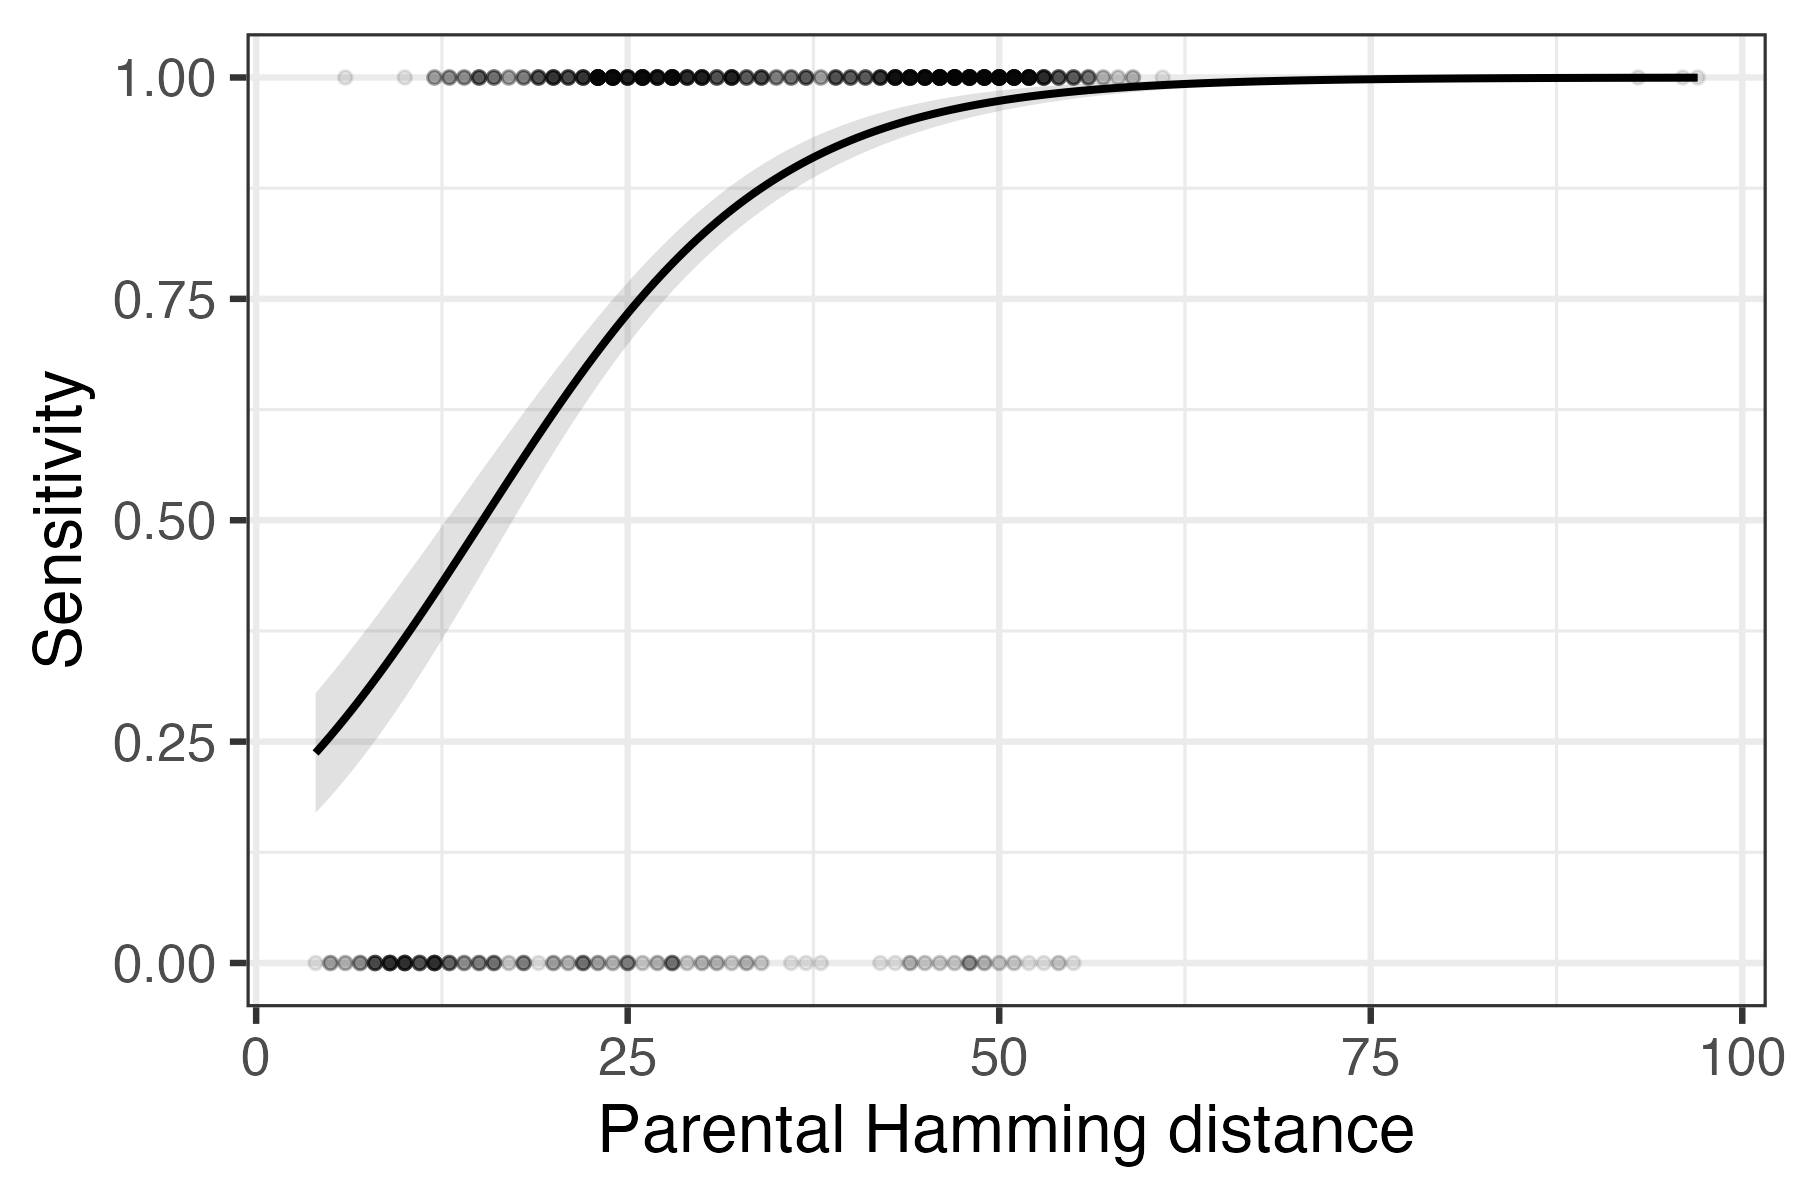
\includegraphics[width=0.8\textwidth]{figures/hmm/sens_vs_parentdist_ggplot.png}
  \caption[Sensitivity dist]{
    Sensitivity to detect recombinants as a function of the Hamming distance between their two parental sequences. The black line represents the logistic regression fit. The grey band represents pointwise Wald 95\% CIs. 
  }
  \label{fig:sens_vs_edits}
\end{figure}

To assess breakpoint resolution, we evaluated the accuracy of inferred breakpoint positions for recombinant sequences. We define the breakpoint distance as the absolute difference in genomic position between true and inferred recombination breakpoints. 

Among sequences with one breakpoint (that had one inferred breakpoint), the mean breakpoint distance was 1,238 nucleotides (95\% CI: [1,108, 1,386]). For sequences with two breakpoints (that had two inferred breakpoints), the mean breakpoint distance was 1,007 nucleotides (95\% CI: [901, 1,125]). For synthetic recombinants with two true breakpoints, we ordered true and detected breakpoints 5' to 3', paired them positionally (1st with 1st, 2nd with 2nd), and calculated the distance between each pair. We then took the average across all paired distances. 

It is difficult to assess breakpoint resolution for a recombinant sequence whose inferred breakpoint count does not match its true breakpoint count. A confusion matrix of inferred and true breakpoint counts for recombinant sequences is shown in Table \ref{tab:bp_confusion}.

\begin{table}[htbp]
\centering
\footnotesize
\begin{tabular}{@{}lrrrr@{}}
\toprule
\multicolumn{1}{c}{\textbf{True breakpoints}} &
\multicolumn{4}{c}{\textbf{Inferred breakpoints}} \\ \cmidrule(l){2-5}
 & 0 & 1 & 2 & 3 \\ \midrule
1 & 77 & 417 &   6 &  0 \\
2 & 122 &  119 & 256 &  3 \\ \bottomrule
\end{tabular}
\caption[Confusion matrix of inferred versus true breakpoint counts]{Confusion matrix of inferred versus true breakpoint counts.}
\label{tab:bp_confusion}
\end{table}

\subsection{Real data analysis} 

We used our method to predict the local Pango lineage ancestry for 440,307 SARS-CoV-2 sequences collected in England between September 2020 and March 2024. These sequences were sampled across 185 test windows that each consisted of a 7-day period with no gaps between successive windows. Of the 440,307 sequences, 7,619 were detected to be recombinant sequences using our method, which corresponds to 1.73\% (95\% CI: [1.69\%, 1.77\%]) of the sequences. 

In Figure \ref{fig:freq2}, we plot the estimated recombinant proportion (the proportion of tested sequences inferred to be recombinant) in each test window and the SARS-CoV-2 prevalence estimates from the ONS survey averaged within each test window. We see a positive trend in the estimated recombinant proportion over time. Our confidence intervals widen in later windows because fewer sequences are available for analysis.

% Our method is only able to detect recombinants whose parents belong to different Pango lineages, and the number of Pango lineages is higher in later test windows. Thus, the proportion of recombinants that are detectable using our method is likely higher in later test windows. 

\begin{figure}[H]
\centering
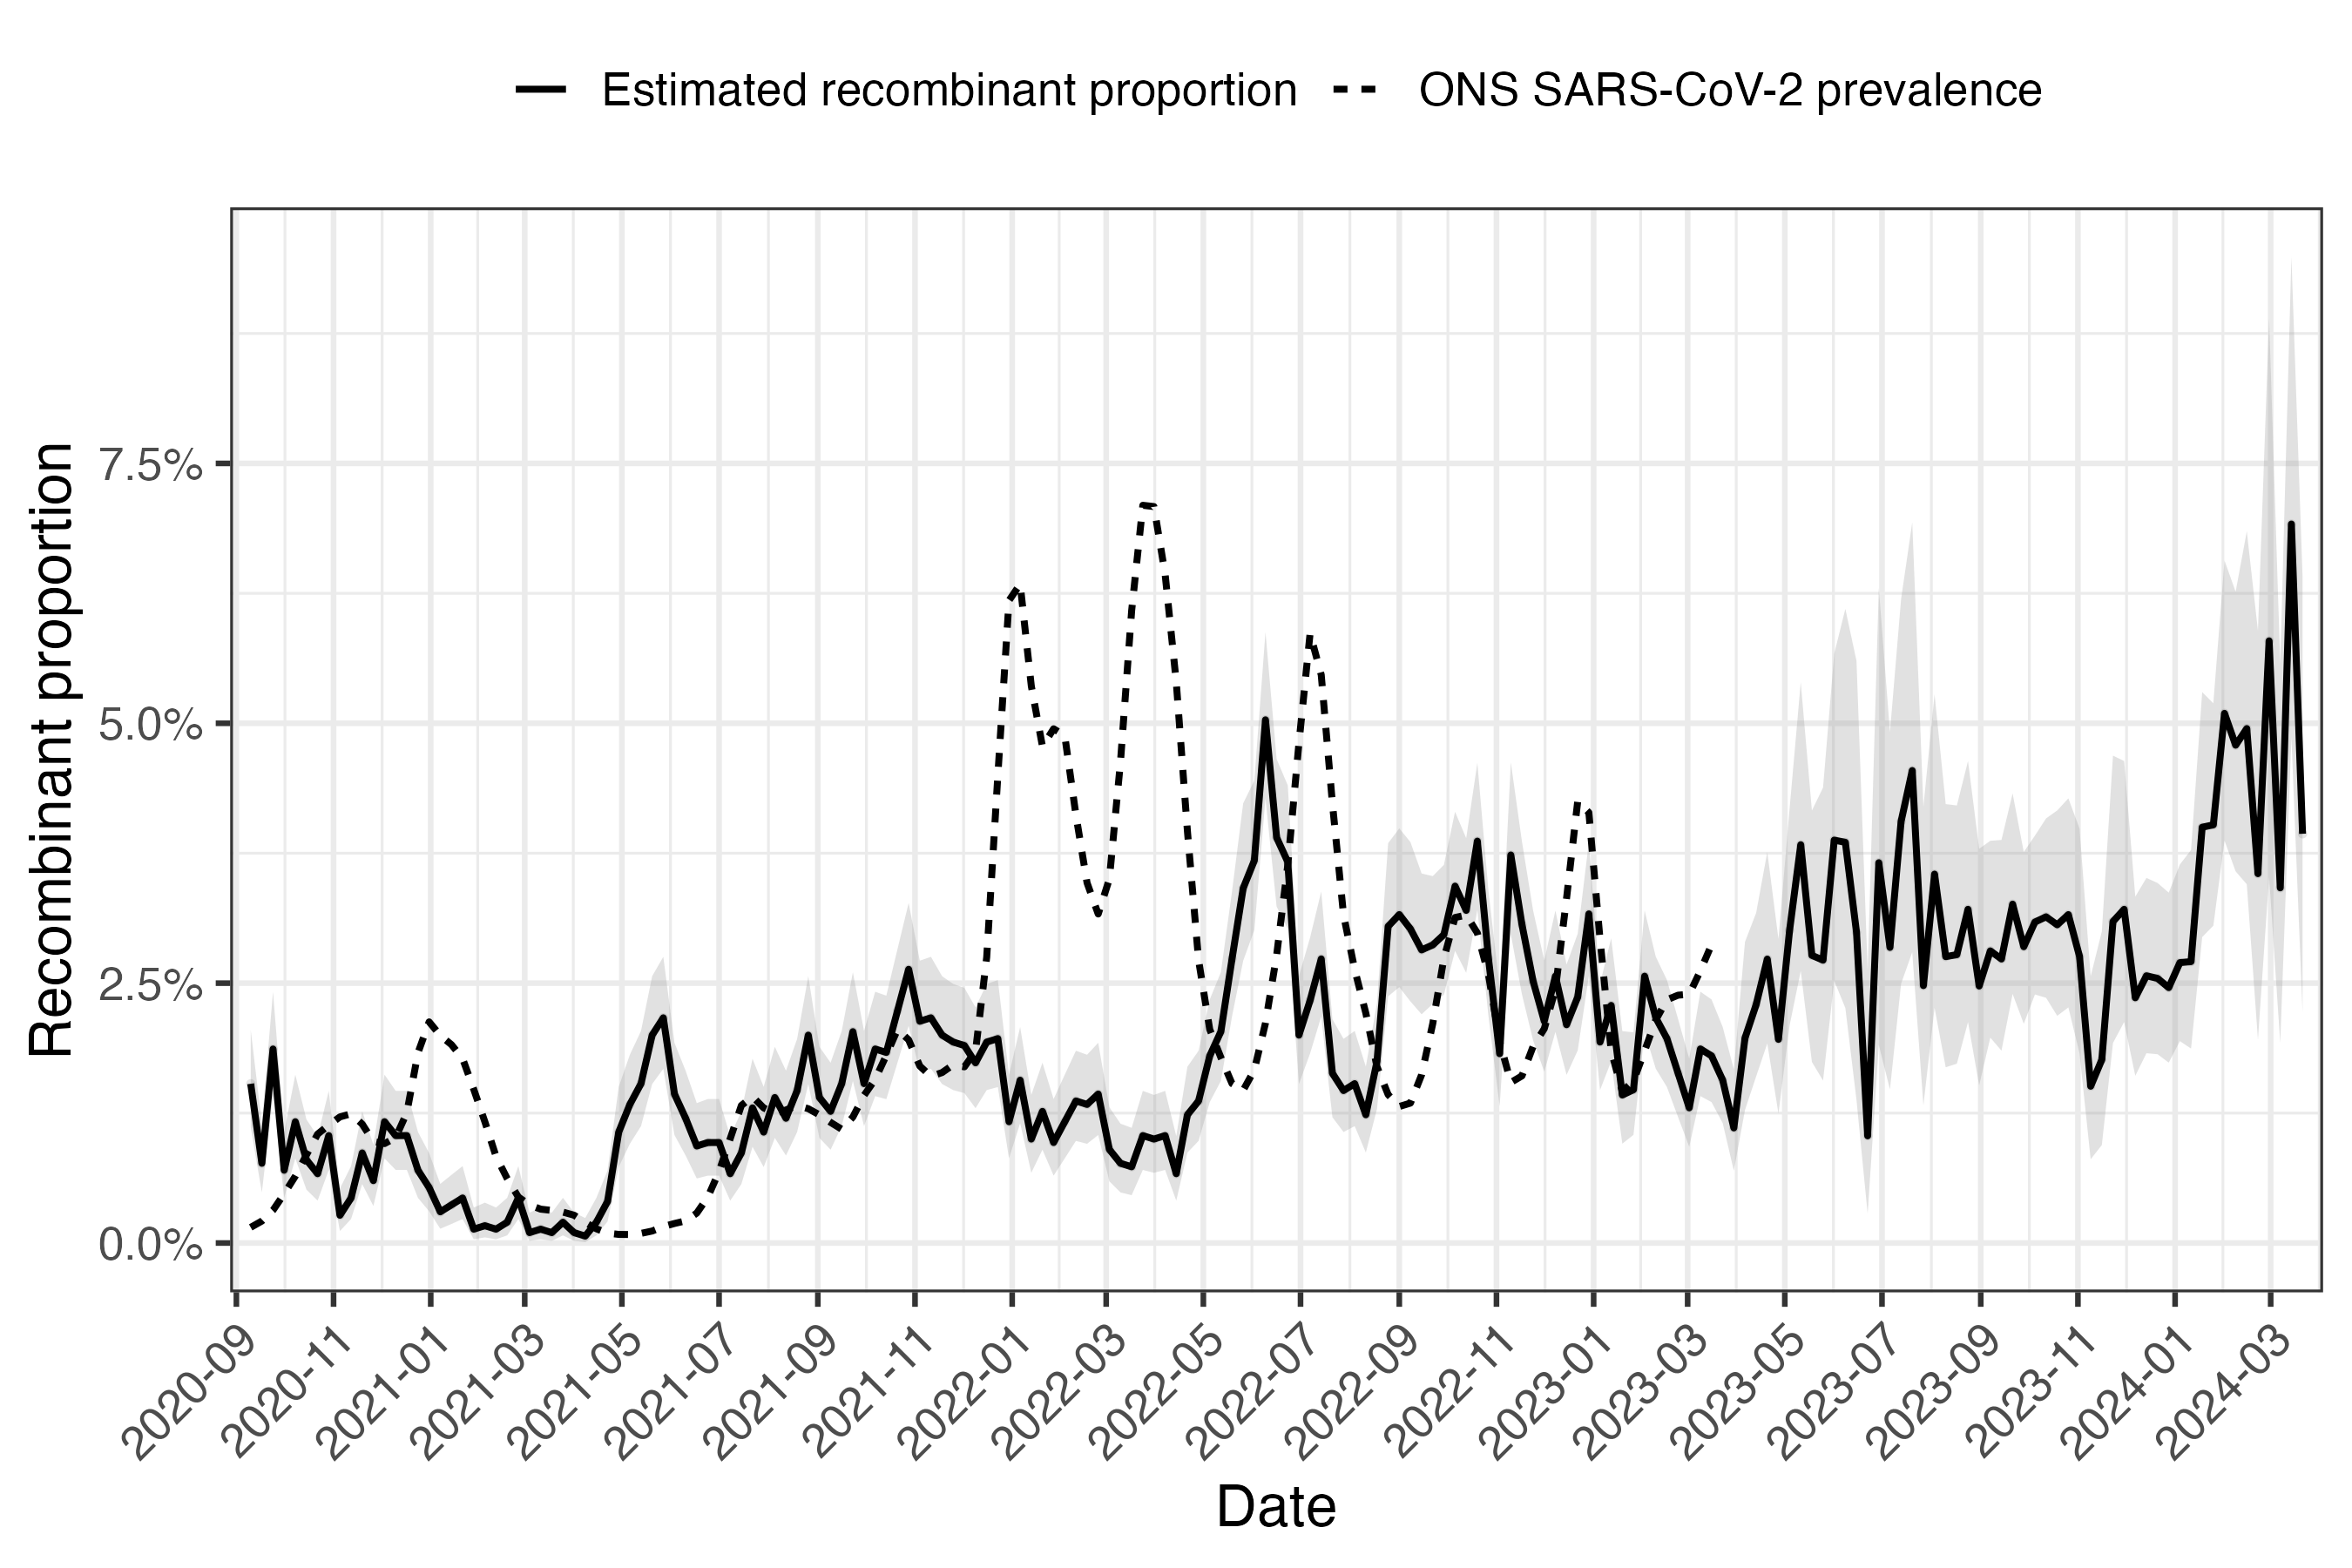
\includegraphics[width=\textwidth]{figures/hmm/line_plot.png}
\caption[Estimated recombinant proportion and ONS prevalence estimates]{Estimated recombinant proportion and ONS prevalence estimates across test windows. The solid line shows the estimated recombinant proportion in each test window. The shaded band indicates 95\% exact binomial confidence intervals for the recombinant proportion in each test window. The dashed line shows daily SARS-CoV-2 prevalence estimates from the ONS survey averaged within each test window.}
\label{fig:freq2}
\end{figure}

The estimated recombinant proportion was positively associated with SARS-CoV-2 prevalence estimates from the ONS survey, averaged within each test window ($p=0.0436$ using a two-sided Pearson correlation test). Figure \ref{fig:scatter} shows the estimated recombinant proportion against the window-averaged prevalence estimates. We label windows with averaged prevalence estimates $>6\%$ with their midpoint date. High prevalence windows correspond to late 2021 and early 2022, when ONS prevalence estimates greatly exceeded the estimated recombinant proportion (see Figure \ref{fig:freq2}). ONS prevalence estimates were available for the first 132 of 185 test windows (until the window ending March 19, 2023). These windows were used to compute the Pearson correlation and $p$-value in Figure \ref{fig:scatter}.

\begin{figure}[H]
\centering
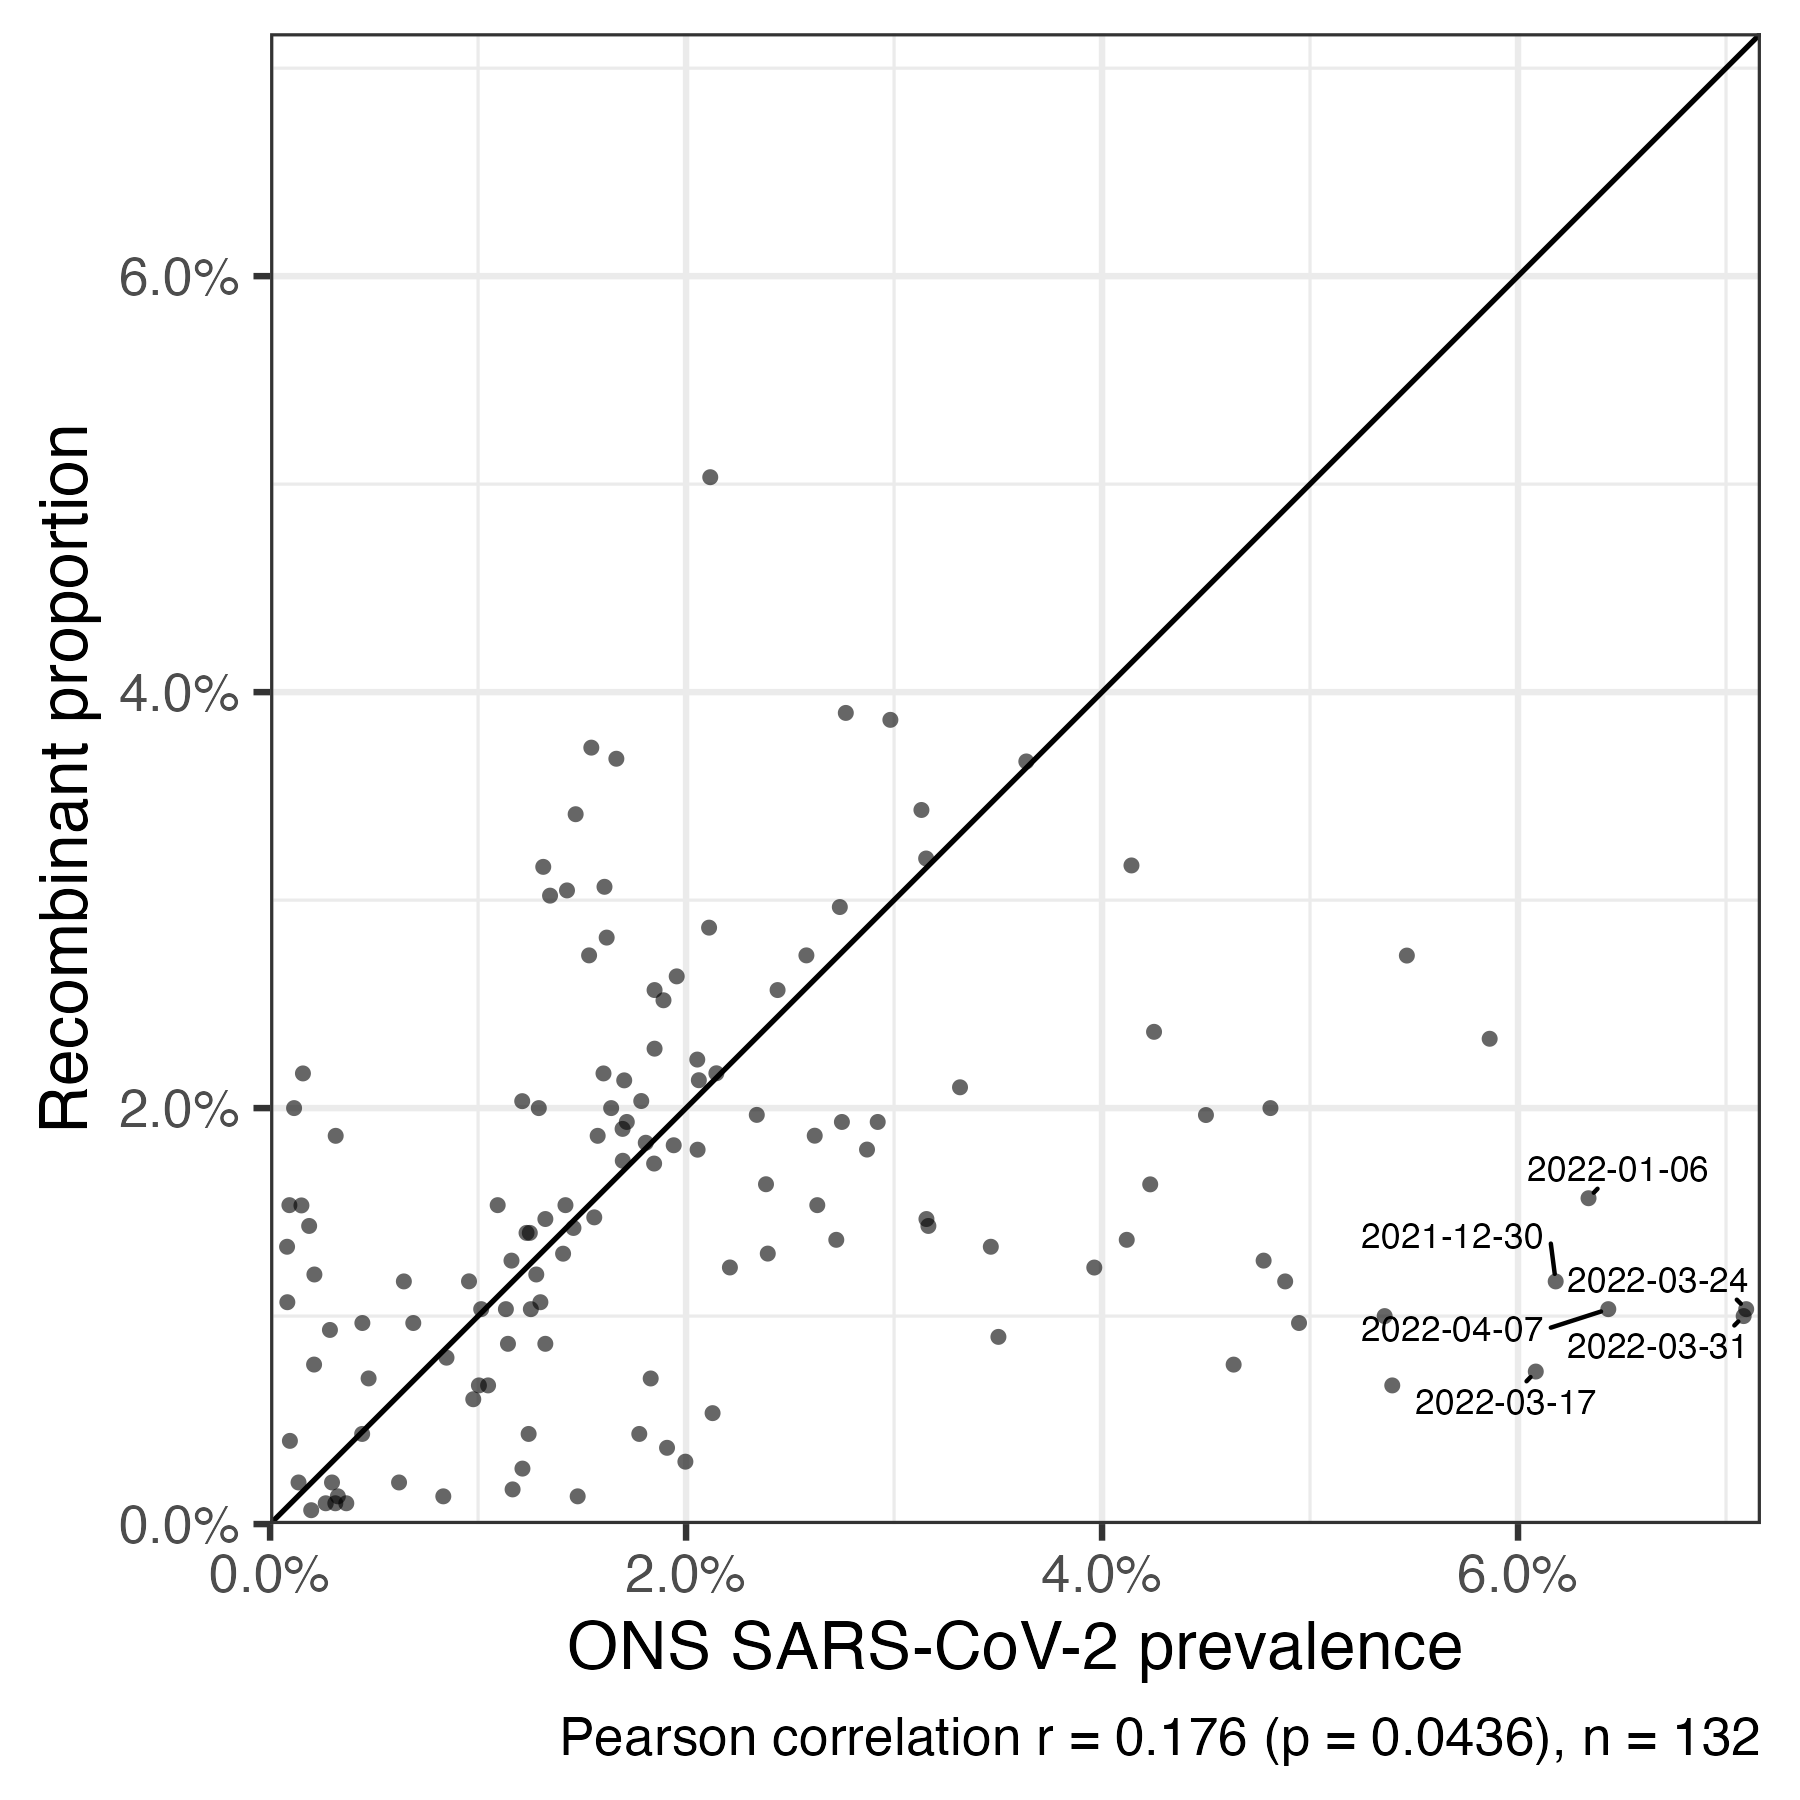
\includegraphics[width=0.8\textwidth]{figures/hmm/scatter_prop_vs_ons.png}
\caption[Scatter: recombinant proportion vs ONS prevalence]{Scatterplot of estimated recombinant proportion against ONS prevalence estimates across test windows. Each point represents one test window. The diagonal line is the identity $y=x$. Windows with averaged prevalence estimates above 6\% are annotated with their midpoint date. The reported $p$-value ($p=0.0436$) is from a two-sided Pearson correlation test.}
\label{fig:scatter}
\end{figure}

Of the 7,619 detected recombinants, 7,063 had exactly two parental lineages in the inferred local Pango lineage ancestry, corresponding to 92.7\% (95\% CI: [92.1\%, 93.3\%]) of detected recombinants. We counted the number of detected recombinants stratified by unique parental lineage pairs. For each parental lineage pair $i<j$, we compared the number of detected $i\text{--}j$ recombinants  (excluding cases in which one of the parental lineages was in the ``other" category) to $\hat{\mathrm{E}}[R_{i,j}]$ derived in Section \ref{sec:expected}, which represents our estimate of the expected number of true positive $i\text{--}j$ recombinants detected across all test windows. For brevity, we henceforth refer to $\hat{\mathrm{E}}[R_{i,j}]$ as the expected TP (true positive) count for $i\text{--}j$ recombinants.

ONS SARS-CoV-2 prevalence estimates are used to obtain expected TP counts for each lineage pair $i<j$. For comparability with these counts, detected recombinant counts are also restricted to windows with available ONS prevalence estimates (until the window ending March 19, 2023). For reference, test windows before March 19, 2023 contained 387,054 sequences, with 5,006 sequences detected as recombinant with exactly two parental lineages in their inferred local Pango lineage ancestry (excluding cases in which one of the parental lineages were in the ``other" category, see Section \ref{subsec:data}). 

% Of these 5,650 sequences, 5,006 sequences did not have a parental lineage in the ``other" category. 

Across parental lineage pairs $i<j$, the number of detected $i\text{--}j$ recombinants was positively associated with their expected TP counts ($p = 8.88 \times 10^{-22}$ using a two-sided Pearson correlation test). We visualized this association in Figure \ref{fig:scatter2}. 

\begin{figure}[H]
\centering
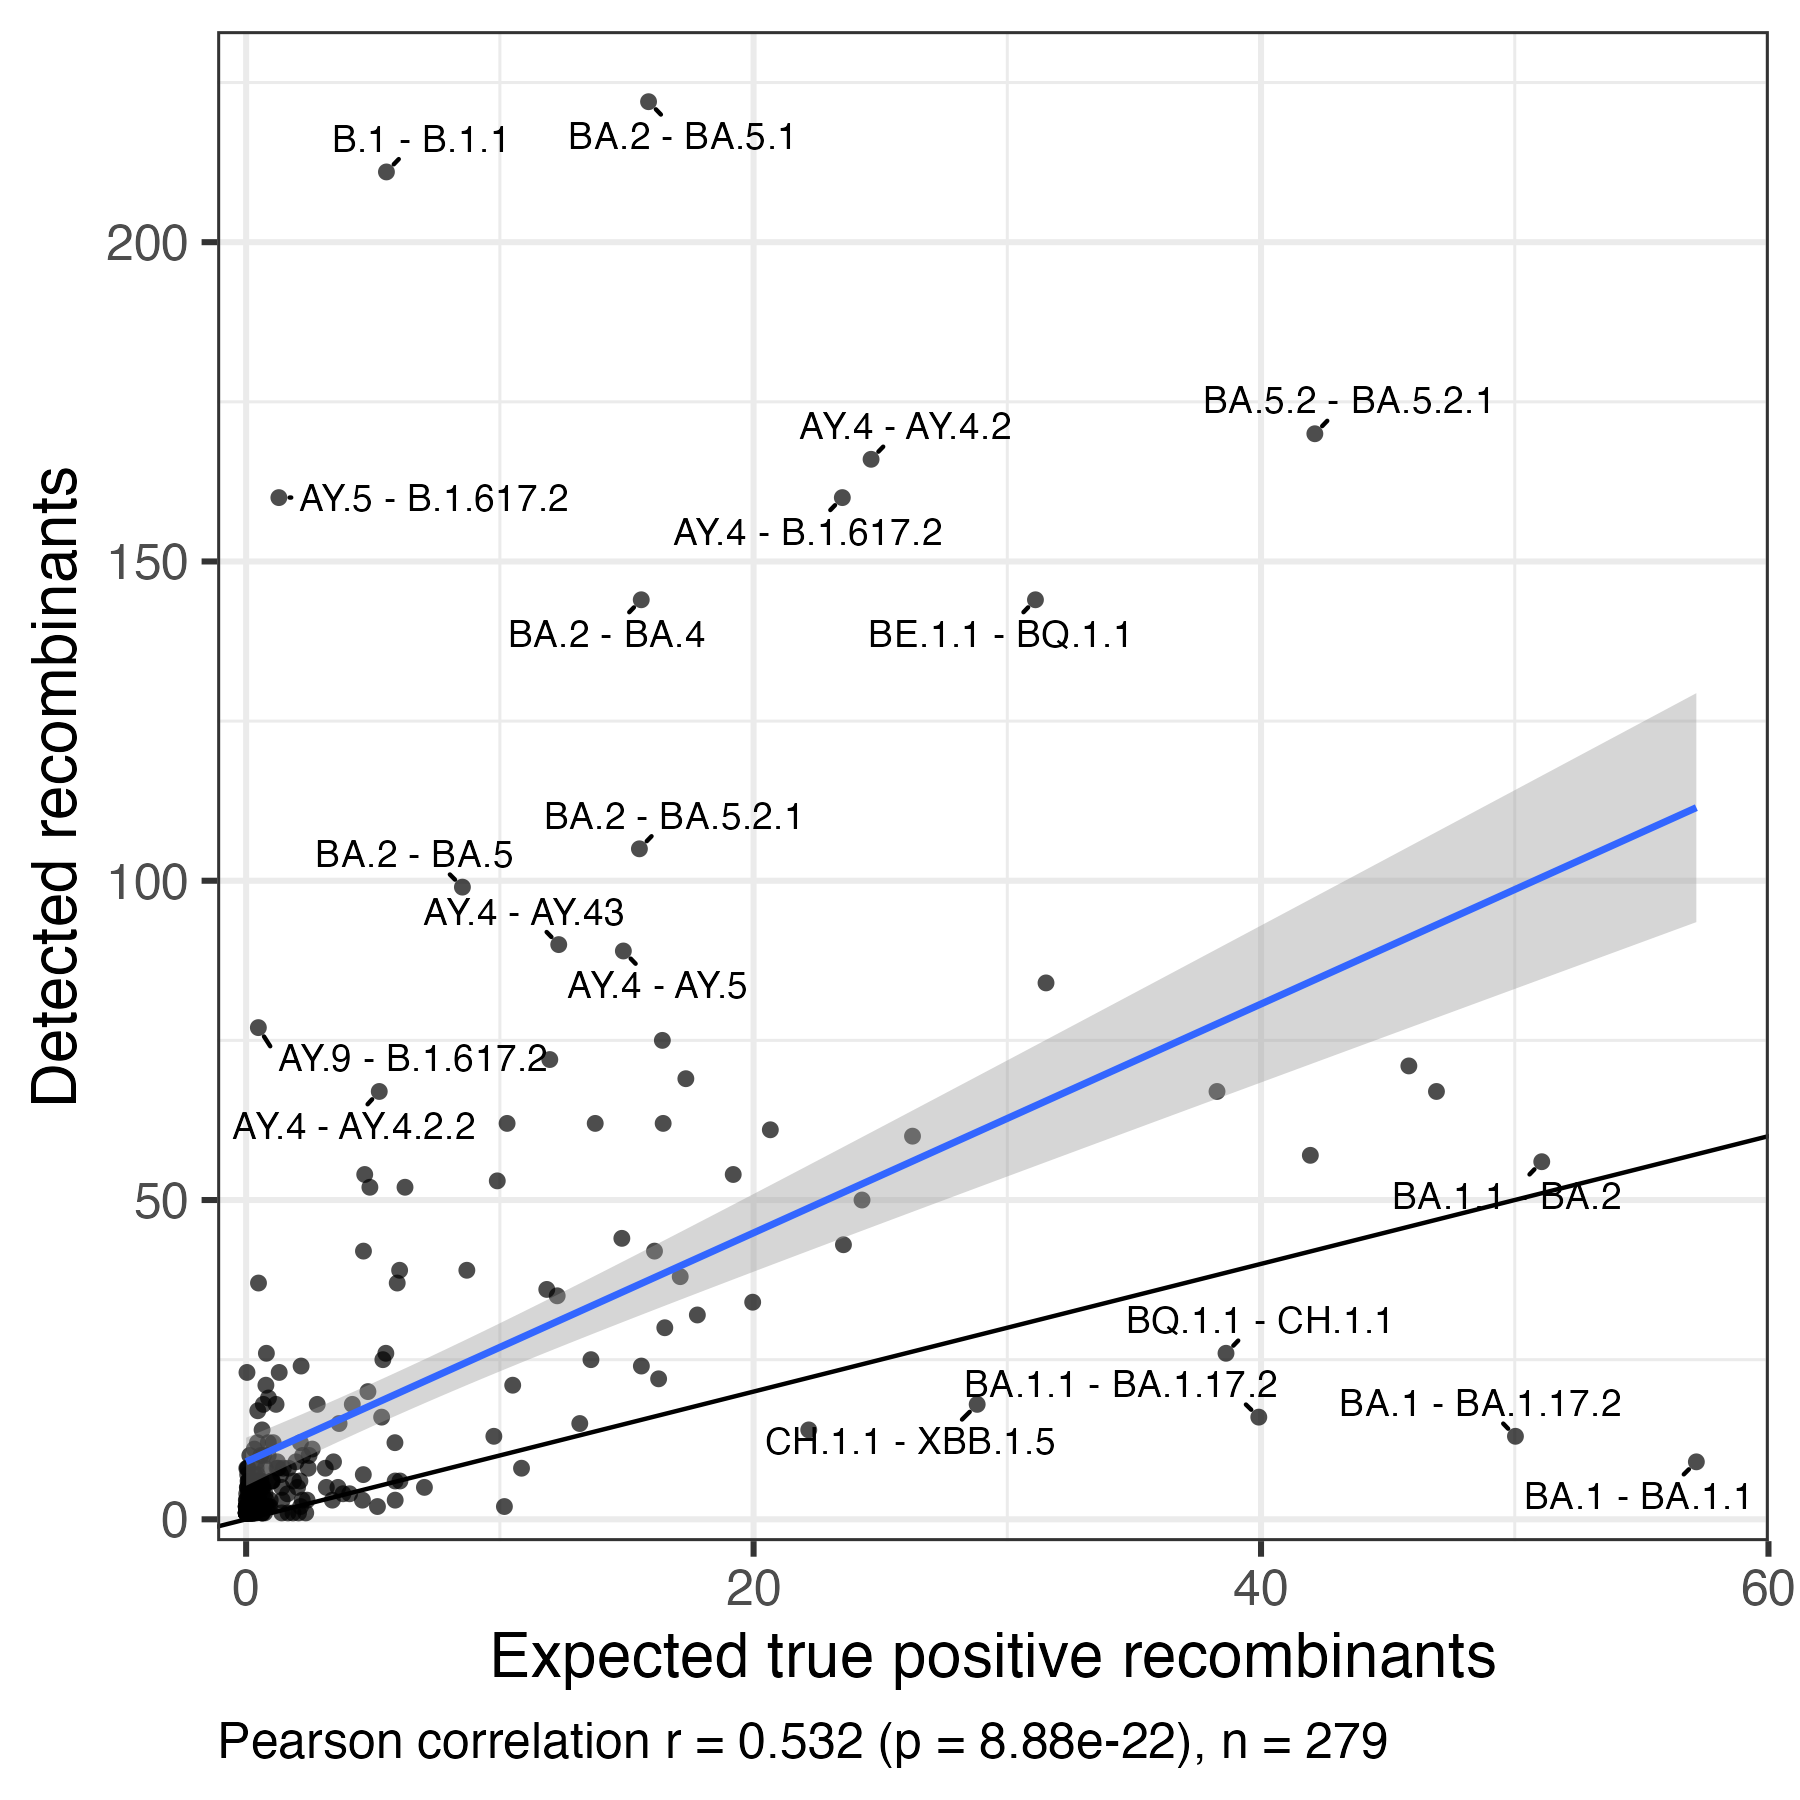
\includegraphics[width=0.8\textwidth]{figures/hmm/pairs_scatter_detected_vs_expected.png}
\caption[Scatter2]{Scatterplot of detected recombinant counts against expected TP counts ($\hat{\mathrm{E}}[R_{i,j}]$). Each point represents a parental lineage pair. The blue line shows the least squares fit with the grey band indicating 95\% confidence intervals for the fitted mean. The black line is the identity $y = x$. We label the 20 parental lineage pairs with the highest absolute residual values from ordinary least squares.}
\label{fig:scatter2}
\end{figure}

Because expected TP counts do not include contributions from false positives, we generally expect the number of detected recombinants to be larger across parental lineage pairs $i < j$. We observe this in Figure \ref{fig:scatter2} (most points fall above the identity line $y = x$). 

Some parental lineage pairs are markedly over- or under-represented relative to the overall trend between detected counts and expected TP counts. To identify these parental lineage pairs, we fit a least squares line with the detected count as the response and the expected TP count as the predictor. We identified the 20 parental lineage pairs with the highest absolute residual values and annotated them in Figure \ref{fig:scatter2}. 

% We identified the ten parental lineage pairs with the highest absolute standardized residuals, which were B.1--B.1.1, BA.2--BA.5.1, AY.5--B.1.617.2, AY.4--AY.4.2, AY.4--B.1.617.2, BA.1--BA.1.1, BA.2--BA.4, BA.1--BA.1.17.2, BA.5.2--BA.5.2.1, and BE.1.1--BQ.1.1 in descending order. These pairs are annotated in Figure \ref{fig:scatter2}. 

Six of these parental lineage pairs had negative residual values. We refer to these parental lineage pairs as under-represented lineage pairs. Recombinants with these parental lineage pairs (except for BA.1.1--BA.2) had lower detected counts than their expected TP counts (these recombinants fall below the identity line $y = x$ in Figure \ref{fig:scatter2}). These findings should be interpreted with caution. The apparent under-representation may be attributable to uncertainty in expected TP counts or sampling variability in detected counts. Alternatively, this may suggest recombinants with these parental lineage pairs occur less frequently in the population than predicted or we have lower sensitivity to detect these recombinants (see Section \ref{sec:expected}). 

We likely have low sensitivity to detect BA.1--BA.1.1, BA.1--BA.1.17.2, and BA.1.1--BA.1.17.2 recombinants, given that only a few mutations separate these lineage pairs. Using consensus sequences and ignoring non-standard nucleotides, pairwise Hamming distances were one for BA.1--BA.1.1, three for BA.1--BA.1.17.2, and four for BA.1.1--BA.1.17.2. Recall that in our simulation study, the sensitivity of our method was low when parental sequences only differed by a few mutations (see Figure \ref{fig:sens_vs_edits}).

Pairwise Hamming distances were relatively high for BQ.1.1--CH.1.1, BA.1.1--BA.2, and CH.1.1--XBB.1.5. However, the sensitivity to detect recombinants with these parental lineage pairs may still be low, depending on where recombinantion breakpoints occur (e.g., the resulting recombinant sequence may only have a few mutations relative to one of its parents, if most of its genome is inherited from this parent). Furthermore, these parental lineage pairs lie close to the identity line $y = x$ (slightly above the line for BA.1.1--BA.2). Thus, their under-representation may be explained by uncertainty in expected TP counts or detected counts.

Interestingly, every under-represented parental lineage pair co-circulated in England during two intervals, late 2021 to early 2022 (BA.1--BA.1.1, BA.1--BA.1.17.2, BA.1.1--BA.1.17.2, BA.1.1--BA.2) and late 2022 to early 2023 (BQ.1.1--CH.1.1, CH.1.1--XBB.1.5), precisely when the estimated recombinant proportion was low relative to ONS prevalence (see Figure \ref{fig:freq2}). For under-represented parental lineage pairs, Figure \ref{fig:freq_pair} shows the pairwise product of their lineage frequencies across test windows. Recombinants with these parental lineage pairs had low detected counts during these two periods, indicating that these under-represented lineage pairs contributed to the lower frequency of recombinants detected during this period. However, further work is needed to determine the cause of this apparent under-representation. 

% Figure \ref{fig:exp_traj} shows expected TP counts across test windows for each under-represented lineage pair. These expected counts scale with the product of lineage frequencies $\hat p_i(w) \hat p_j(w)$ (see Section \ref{sec:expected}), so expected counts for parental lineage pairs are elevated during periods of co-circulation between these pairs.

\begin{figure}[H]
\centering
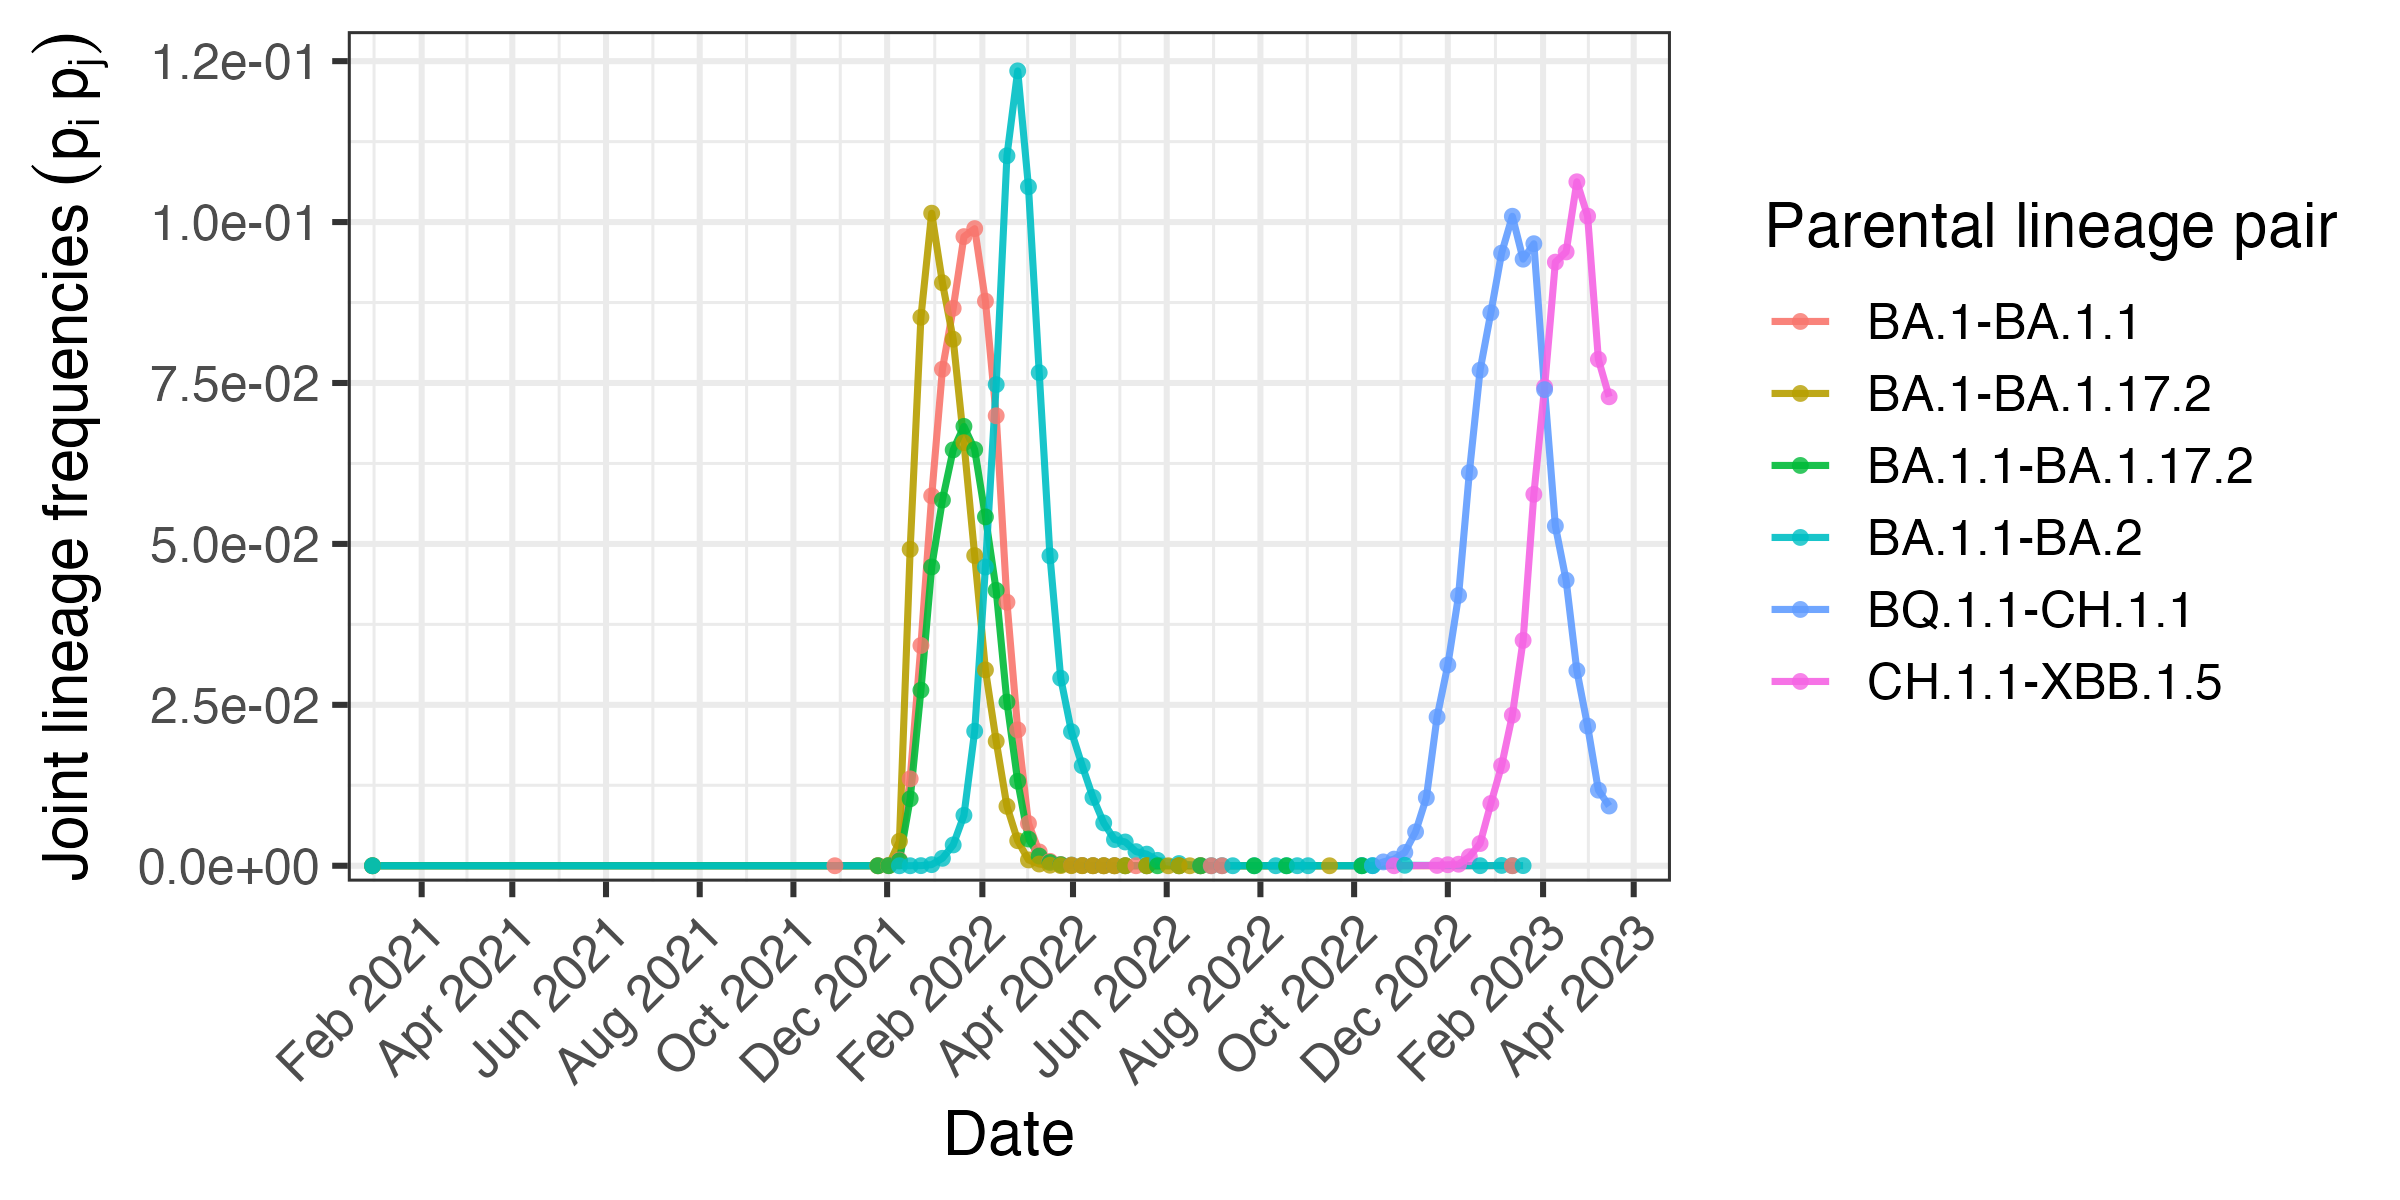
\includegraphics[width=\textwidth]{figures/hmm/pipj_selected_pairs.png}
\caption[traj]{Joint frequencies across test windows for under-represented lineage pairs.}
\label{fig:freq_pair}
\end{figure}

Out of the 20 flagged recombinant pairs with the highest residual values (see Figure \ref{fig:scatter2}), 14 parental lineage pairs had positive residual values, indicating that recombinants with these lineage pairs were detected more frequently relative to the overall trend between detected counts and expected TP counts. It is difficult to pinpoint whether this reflects the population frequency of recombinant sequences with these parental lineage pairs, higher detection sensitivity, disproportionate false positive assignments to these parental lineage pairs, or some combination of these factors.

In the process of estimating expected TP counts, we estimated the detection factor $\theta$ and false positive rate $\phi$ to be 0.557 (95\% CI: [0.309, 0.804]) and 0.011 (95\% CI: [0.009, 0.013]) respectively. Recall that $\theta$ equals sensitivity times the probability that a sample from a co-infected individual is a recombinant (see Section \ref{sec:expected}). Confidence intervals are Wald intervals from the linear regression described in Section \ref{sec:expected}, treating $x_w$ as fixed. Remarkably, our estimated false positive rate closely matches what we estimated in the simulation (see Section \ref{sec:sim_res}).

% Taking detected recombinants with two predicted parental lineages, we plotted their counts and proportions by parental lineage combination across all test windows in Figure \ref{fig:pair_time}. In this figure, we color only the top 18 Pango lineages by proportion summed across test windows to reduce visual clutter. All remaining lineages are shown in grey. Recombinants with at least one parent from these grey lineages are also represented in grey, rather than with a combination of two colors.

% \begin{figure}[H]
% \centering
% 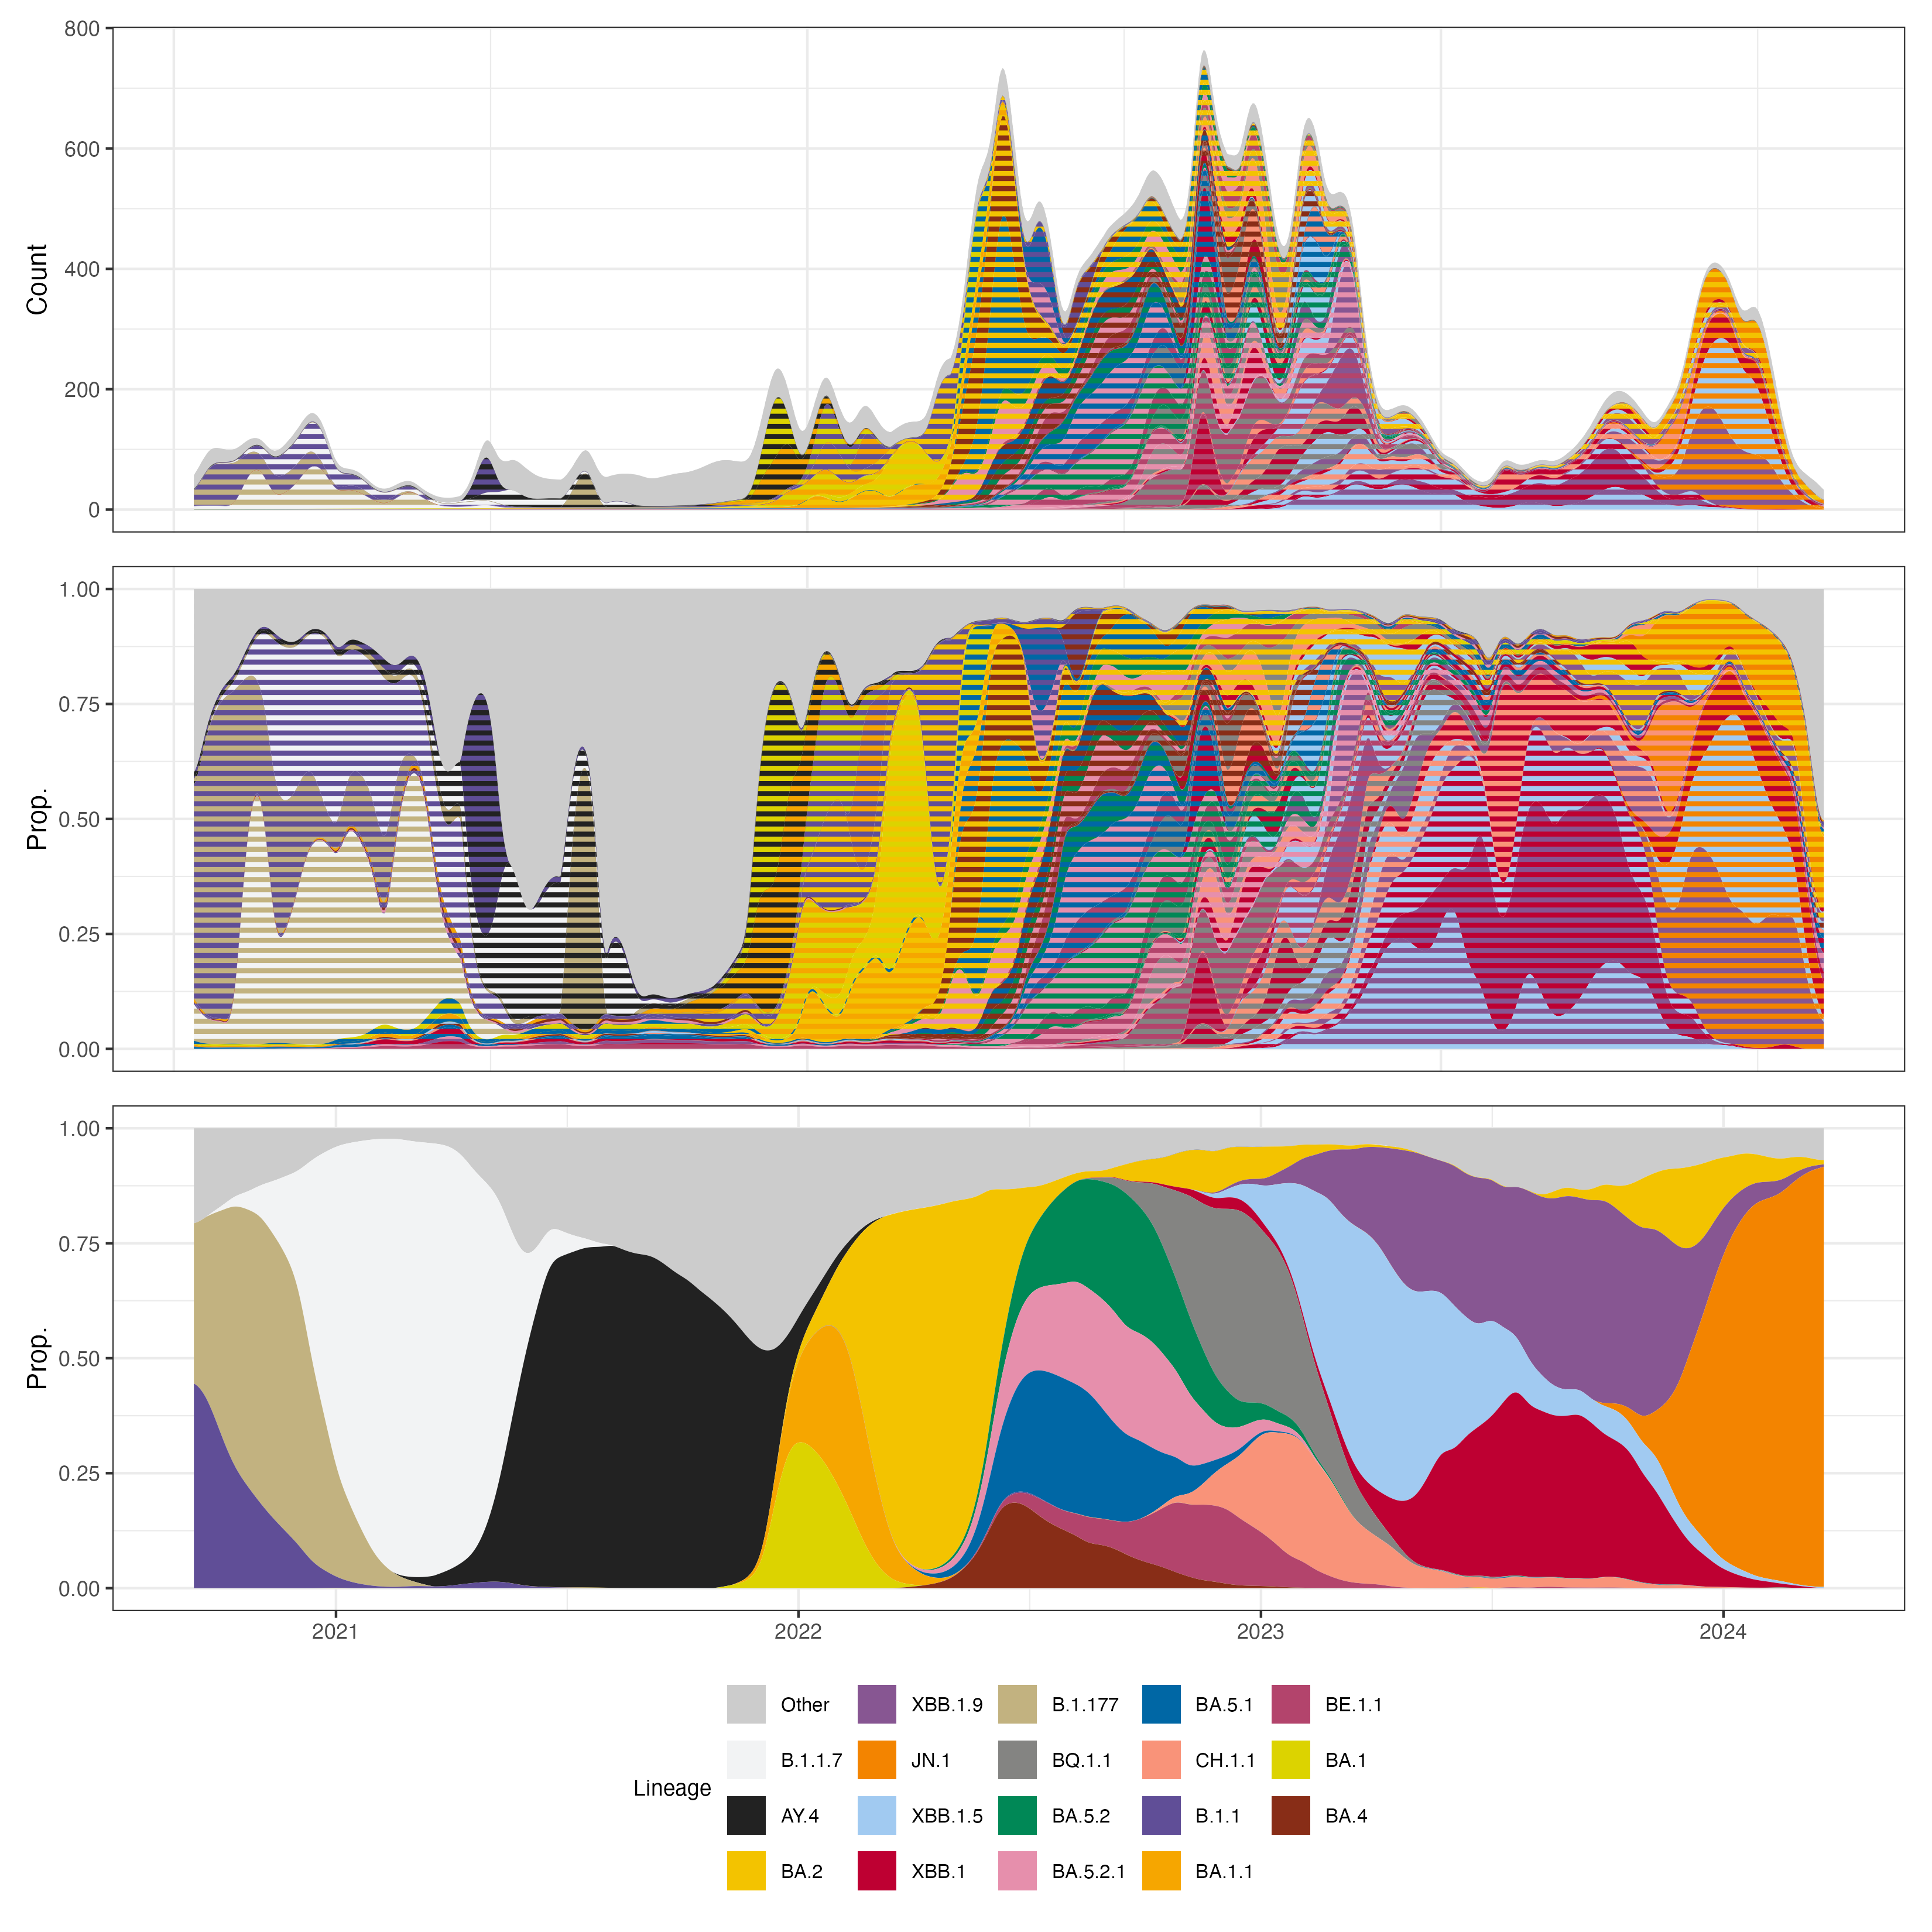
\includegraphics[width=0.9\textwidth]{figures/hmm/streamplot_pairs.png}
% \caption[Counts and proportions of detected recombinant sequences with two predicted lineage combinations]{Counts and proportions of detected recombinant sequences with two predicted lineage combinations. The bottom panel shows the frequency of each Pango lineage across time. The middle panel shows the proportion of detected recombinants with each predicted parental lineage combination. To indicate lineage combinations, we use striped colors comprised of the two lineages contributing ancestry. Finally, the top panel represents the number of detected recombinants with each predicted lineage combination. To avoid using too many colors, we highlighted the top 18 Pango lineages in terms of their frequency summed across test windows. We smoothed each lineage trajectory with a cubic smoothing spline to dampen small week-to-week variations in the counts and proportions.}
% \label{fig:pair_time}
% \end{figure}

Across 7,619 detected recombinants, we detected 9,105 recombination breakpoints. 6,324 (83.0\%) had 1 breakpoint, 1,146 (15.0\%) had 2, 118 (1.5\%) had 3, 23 (0.3\%) had 4, and 8 (0.1\%) had $\geq 5$. In Figure \ref{fig:hist}, we plot the genomic position of each detected breakpoint. We observed localized clusters of recombination breakpoints within Spike and enrichment of breakpoints at the ends of the genome.

\begin{figure}[H]
\centering
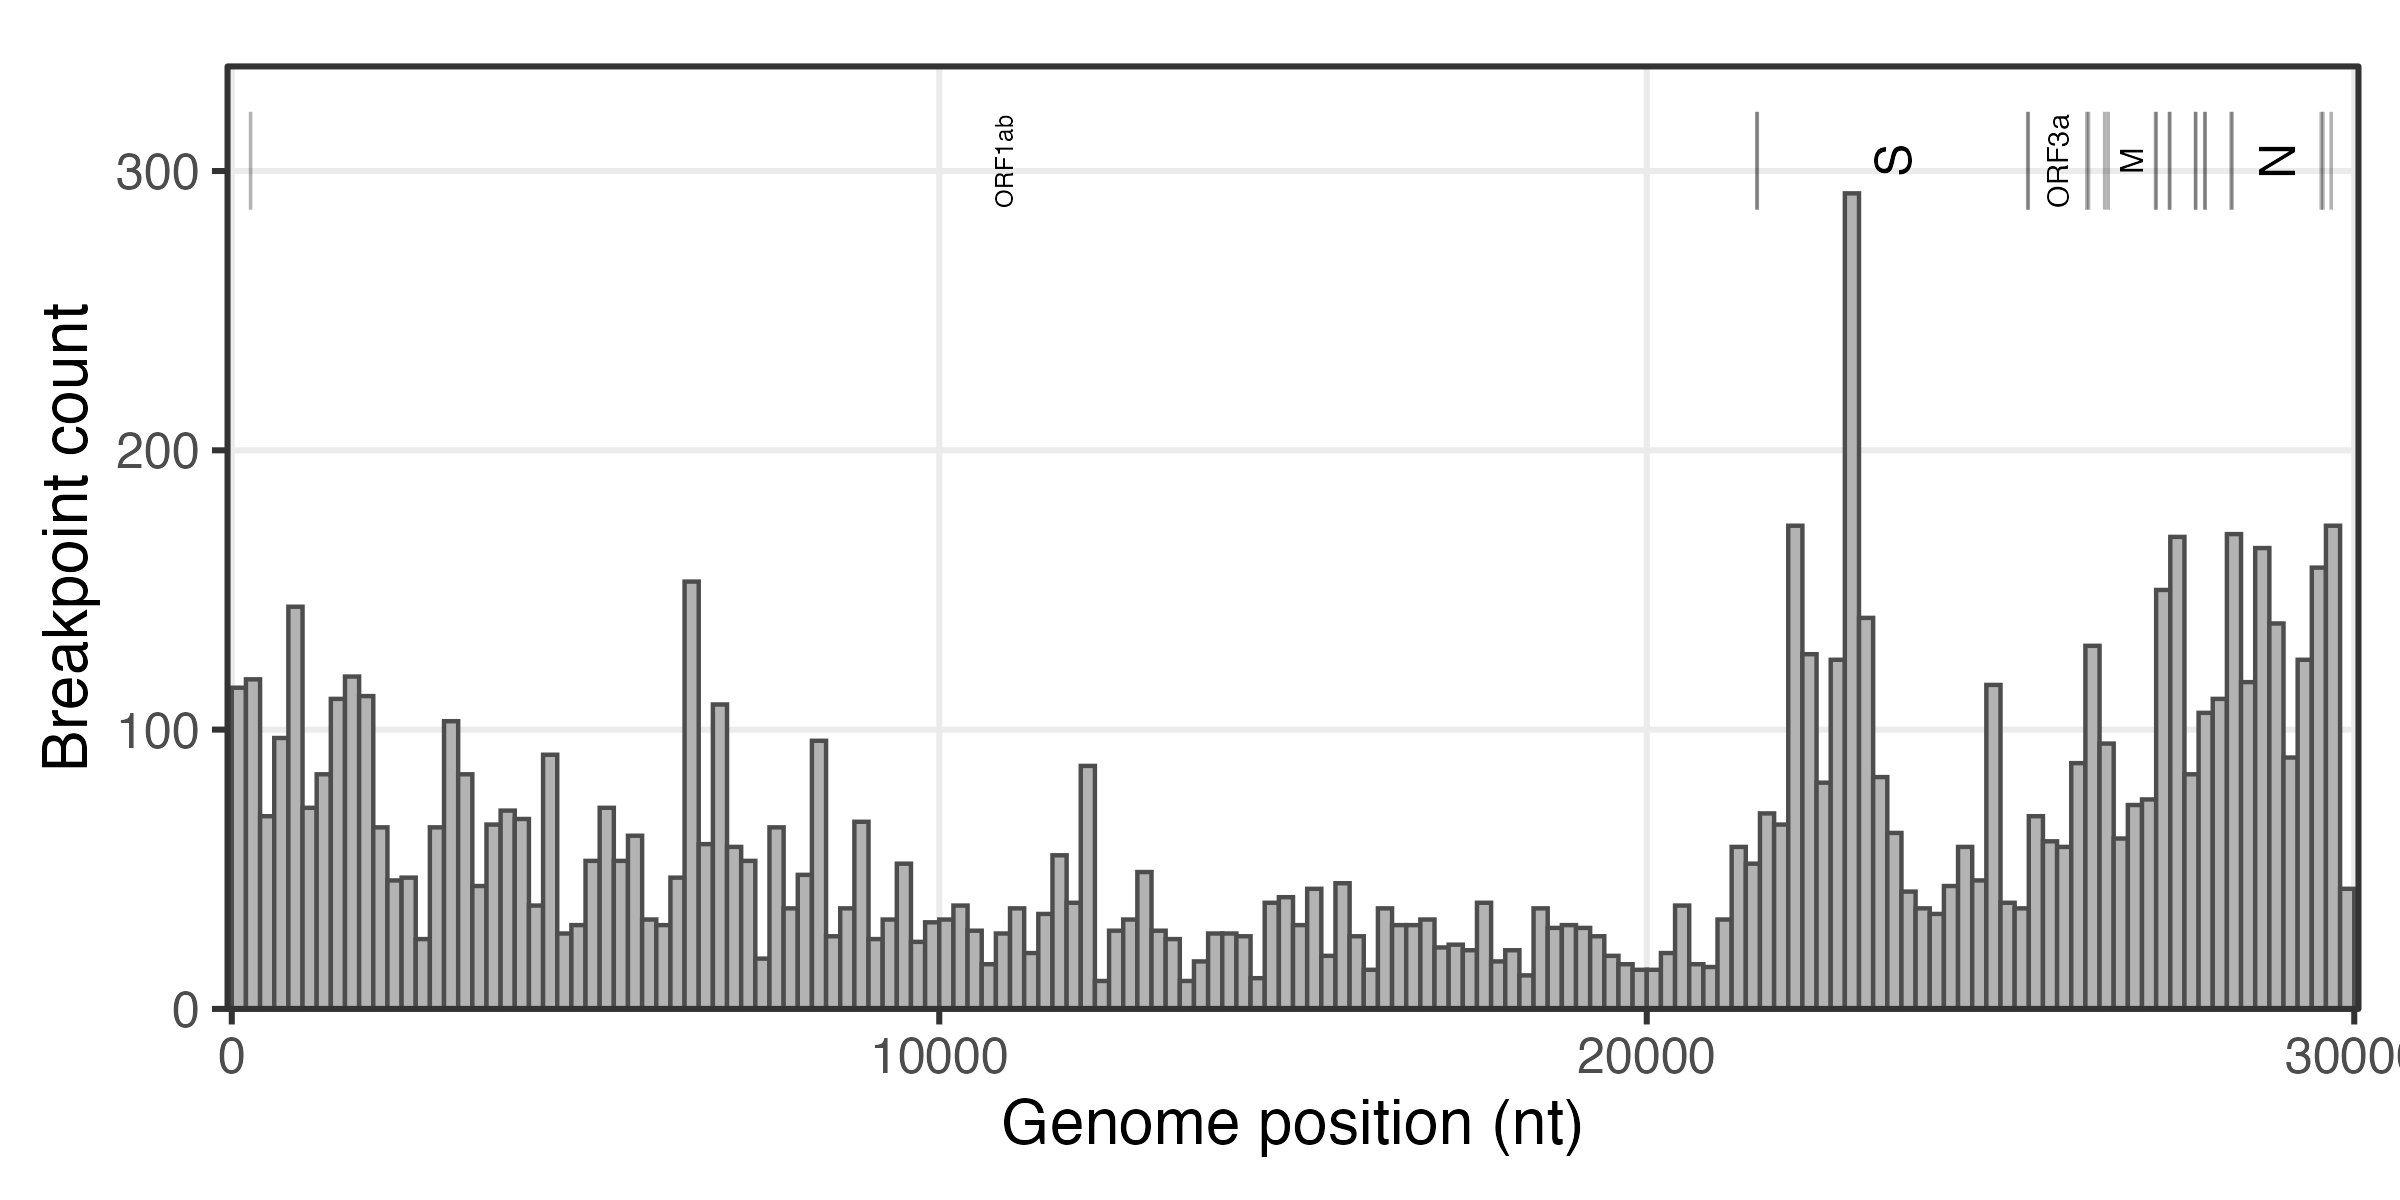
\includegraphics[width=\textwidth]{figures/hmm/recomb_hist_with_gene_intervals.png}
\caption[Histogram of detected recombination breakpoints]{Histogram of detected recombination breakpoints.}
\label{fig:hist}
\end{figure}

We also observed an enrichment of recombination breakpoints in intergenic regions. Although intergenic regions comprise only around 0.5\% of the genome, 1.1\% of all breakpoints were localized in these regions (99/8,767). When calculating the proportion of detected breakpoints in intergenic regions, we excluded 338 breakpoints mapping to the ends of the genome, specifically from the 5' end to ORF1ab and from ORF10 to the 3' end. Using a two-sided binomial test, we found this enrichment to be highly statistically significant ($p = 1.64\times 10^{12}$).

\section{Discussion}

Genetic surveillance of recombinant SARS-CoV-2 sequences is important, given that mutations from each of the parental lineages can provide a growth advantage to the recombinant sequence. In this study, we developed a HMM to detect the local Pango lineage ancestry of query SARS-CoV-2 sequences based on  nucleotide frequencies calculated using a reference set of recent sequences. Our method does not depend on an existing phylogeny nor any user-defined parameters such as the mutation rate or recombination rate. Instead, we use maximum likelihood to estimate the lineage-transition probability between consecutive sites, and the probability of observing alleles absent from the lineage providing ancestry at each site, which accounts for mutations on the recombinant sequence. 

We validated our method using synthetic sequences generated from real SARS-CoV-2 genomes. In our simulation, our method achieved a sensitivity of 0.801 (95\% CI: [0.775, 0.825]) for recombinant sequences and a specificity of 0.989 (95\% CI: [0.980, 0.994]) for non-recombinant sequences. In 69.9\% (95\% CI: [67.0\%, 72.7\%]) of synthetic recombinant sequences, we detected two parental lineages that matched the true parental lineage pair. In 98.4\% (95\% CI: [97.4\%, 99.1\%]) of synthetic control sequences, we detected a single parental lineage that matched the true parental lineage. We found the sensitivity of our method to be strongly positively associated with the number of mutations separating the parental sequences of the recombinant (see Figure \ref{fig:sens_vs_edits}). Finally, we estimated the mean distance between true and inferred breakpoints to be 1,238 nucleotides (95\% CI: [1,108, 1,386]) and 1,007 nucleotides (95\% CI: [901, 1,125]) for synthetic recombinants with one and two breakpoints respectively.

Applying our model to real SARS-CoV-2 sequences collected in England between September 2020 and March 2024, we found 7,619 recombinant sequences across 440,307 sequences, which corresponds to 1.73\% (95\% CI: [1.69\%, 1.77\%]) of sequences. These 440,307 sequences were sampled across 185 test windows, each window corresponding to a 7-day period with no gaps between successive windows. 

We hypothesized that across our test windows, the fraction of tested sequences detected as recombinant using our method would be positively associated with community SARS-CoV-2 prevalence, because higher prevalence raises co-infection opportunities, which should result in a higher rate of recombinant sequences in the population. There was a positive association between the estimated recombinant proportion in each test window and SARS-CoV-2 prevalence estimates from the ONS survey, averaged within each test window ($r = 0.176$, $p = 0.0436$ using a two-sided Pearson correlation test). 

We modeled the number of recombinants in our sample as a function of community SARS-CoV-2 prevalence to derive, for each parental lineage pair, the expected number of true positive recombinants across the 440,307 sequences analyzed (Section \ref{sec:expected}). This derivation relies on two key assumptions. First, we assume independent infections in our co-infection model, which means that the probability of co-infection by two lineages equals the product of their marginal prevalences. Second, we assume that the false positive rate and the detection factor (the product of sensitivity and the probability that a sequence from a co-infected individual is a recombinant) are constant across parental lineage pairs and test windows. Our second assumption ensures identifiability of the false positive rate and detection factor in our model. We estimated the false positive rate and detection factor to be 0.011 (95\% CI: [0.009, 0.013]) and 0.557 (95\% CI: [0.309, 0.804]) respectively for the real data analysis. Our estimated false positive rate closely matched the false positive rate estimated from the simulation study. 

We estimated the expected TP count for each parental lineage pair. We found that the number of detected recombinants with each parental lineage pair exceeded the corresponding expected TP count for most parental lineage pairs. This is not surprising. We expect the vast majority of analyzed sequences (440,307) to be non-recombinants. Based on our estimated false positive rate, we expect approximately 4,400 of the 7,619 detected recombinants to be false positives. However, we cannot reliably allocate expected false positive counts across specific parental lineage pairs.

Recall that during the period when ONS SARS-CoV-2 prevalence estimates were available (until the test window ending Match 19, 2023), we analyzed 387,054 sequences, with 5,006 sequences detected as recombinant with two parental lineages. Using a similar calculation, we expect around 3,800 of these detected recombinants to be false positives. The expected TP count summed across all lineage pairs was 1,390, which is close to the implied TP count ($5006 - 3800 = 1206$). 

Although many detections are likely false positives, across parental lineage pairs, we found a strong positive association between our expected TP estimates and the number of detected recombinants ($r = 0.532$, $p = 8.88\times 10^{-22}$ using a two-sided Pearson correlation test). This indicates that our method is detecting recombinants at a rate that is predictable based on SARS-CoV-2 prevalence and co-infection dynamics between lineages. 

We then identified parental lineage pairs that were over- or under-represented relative to the overall trend between detected counts and expected TP counts. We identified six under-represented parental lineage pairs (BA.1--BA.1.1, BA.1--BA.1.17.2, BA.1.1--BA.1.17.2, BQ.1.1--CH.1.1, BA.1.1--BA.2, CH.1.1--XBB.1.5). These lineage pairs, except for BA.1.1--BA.2, had lower detected counts than expected TP counts. 

Under-representation of BA.1--BA.1.1, BA.1--BA.1.17.2, and BA.1.1--BA.1.17.2 recombinants is likely explained by low sensitivity to detect these recombinants. Only a few mutations separate each of these lineage pairs, making recombinant detection difficult (see Figure \ref{fig:sens_vs_edits}). On the contrary, pairwise Hamming distances are high for BQ.1.1--CH.1.1, BA.1.1--BA.2, and CH.1.1--XBB.1.5. However, if resulting recombinant sequences are very similar to one of their parental lineages (e.g., due to breakpoints localizing to certain positions), the sensitivity to detect these recombinants may still be low. 

Another possibility is that these lineages were circulating in different geographical areas or subpopulations in England, which make co-infection unlikely. Co-infection rates may be lower than expected even under homogeneous mixing, due to within-host interference. Moreover, lineage pairs may differ in their propensity to produce viable recombinants. Finally, the apparent under-representation of these parental lineage pairs could result from estimation error in expected TP counts or sampling variability in detected counts. Estimating the variability of expected TP counts is challenging. We do not have standard errors for ONS SARS-CoV-2 prevalence estimates. Additionally, we must account for correlations in lineage prevalences across test windows. 

We found that these six under-represented lineage pairs co-circulated in England during two intervals, late 2021 to early 2022 (BA.1--BA.1.1, BA.1--BA.1.17.2, BA.1.1--BA.1.17.2, BA.1.1--BA.2) and late 2022 to early 2023 (BQ.1.1--CH.1.1, CH.1.1--XBB.1.5). These two intervals coincide with periods when the estimated recombination proportion was low relative to ONS SARS-CoV-2 prevalence estimates. This indicates that these under-represented lineage pairs contributed to the lower frequency of recombinants during these periods. 

Finally, we observed localized clusters of recombination breakpoints within Spike, which is consistent with previous work on recombination hotspots in sarbecoviruses \cite{lytras_exploring_2022}. 
Additionally, we found that breakpoints were enriched in intergenic regions, consistent with their high colocalization with TRS-B sites \cite{yang_characterizing_2021}.

Using RIPPLES, Turakhia et al. found 2.7\% of sampled genomes inferred to have detectable recombinant ancestry \cite{turakhia_pandemic-scale_2022}. This is higher than the proportion of detected recombinants using our method (1.73\%; 95\% CI: [1.69\%, 1.77\%]). This discrepancy is likely attributable to many factors. Turakhia et al. only analyze sequences up to May 2021, before the emergence of XBB. Furthermore, our method cannot detect recombination between sequences in the same lineage, which explains the lower proportion of detected recombinants using our method. Finally, even a modest difference in false positive rates would affect the estimated proportion.

Future work could estimate SARS-CoV-2 prevalence from the frequency of detected recombinants across test windows. In this study, we developed a statistical framework linking prevalence and the expected number of detected recombinants (see Section \ref{sec:expected}). We further showed that detections were correlated with the product of prevalence and parental lineage frequencies. Thus, estimating prevalence is feasible if the method’s sensitivity and false positive rate were known across different scenarios. In our study, we inferred the detection factor and false positive rate from ONS prevalence estimates (see Section \ref{sec:expected}), so these rates are not generalizable outside England or beyond March 2023, when ONS prevalence estimates are no longer available.

Although we focused on SARS-CoV-2 in this study, our HMM is broadly applicable to other RNA and DNA viruses for detecting recombinants. Moreover, by limiting lineage transitions to predefined genome positions, our HMM can be easily adapted to detect reassortment events in segmented viruses such as influenza. Our detection method should perform well on rapidly evolving viruses because we explicitly model novel alleles on recombinant sequences via a pseudo-frequency. 

\section{Implementation} 

The hidden Markov model and detection of recombinant sequences were implemented in Python 3.12.2. Results files were processed and plotted in R version 4.4.1.

\section{Availability}

All code for the analysis is available at \href{https://github.com/nobuakimasaki/HMM-recombination}{github.com/nobuakimasaki/HMM-recombination}.

\section{Acknowledgments}

We thank Professor Brian Browning for helpful suggestions on accelerating the forward algorithm and Professor Nicola Mueller for discussions of co-infection dynamics.

We gratefully acknowledge the investigators and laboratories that generated, submitted, and shared sequence data and metadata via GenBank (NCBI), which form the basis of this research.


% \section{Author contributions} 

% AR, MAS, TB conceived the study.
% AR, MAS, TB, DJS, PL designed the antigenic model.
% TB, GD, VG, JWM, AJH, CAR, DJS, AR gathered antigenic and genetic data.
% AR, MAS, TB, PL implemented statistical phylogenetic procedures.
% TB, AR performed the analysis.
% TB, AR, DJS, JWM, PL, CAR, AJH, GD, MAS interpreted the results.
% TB, MAS, AR, JWM, AJH wrote the paper.

%%% FUNDING %%%

\section{Funding} 

This work is supported by NIH NIGMS (R35 GM119774 to T.B.). T.B. is a Howard Hughes Medical Institute Investigator.

%%% REFERENCES %%%
\bibliographystyle{plain}
\bibliography{references}

\end{document}